% Copyright (C)  2016 Philipp Hacker.
% Permission is granted to copy, distribute and/or modify this document
% under the terms of the GNU Free Documentation License, Version 1.3
% or any later version published by the Free Software Foundation;
% with no Invariant Sections, no Front-Cover Texts, and no Back-Cover Texts.
% The lincense itself can be found at <https://www.gnu.org/licenses/fdl-1.3>.

\documentclass[a4paper,10pt,twoside]{article}

\usepackage{lipsum}
\usepackage{multicol}

\usepackage[T1]{fontenc}
\usepackage[utf8]{inputenc}

\usepackage[infoshow]{tabularx}
\usepackage[all]{xy}

\usepackage{geometry}
\geometry{%
	a4paper,
	left=24mm,
	right=24mm,
	top=24mm,
	bottom=24mm,
	}

\usepackage{amsmath,mathtools}
\usepackage{amssymb}
\usepackage{units}
\usepackage{upgreek}
\usepackage{graphicx}

\usepackage{float}
\usepackage{lscape}

\usepackage[labelfont=bf]{caption}
\usepackage{wrapfig}
\usepackage{subcaption}

\usepackage[backref=page]{hyperref}

\usepackage{csquotes}
\usepackage[infoshow]{tabularx}
\usepackage{fancyhdr}

\usepackage{sectsty}
\usepackage{times}

\usepackage{lmodern} %TODO Schriftart
\usepackage[greek,english]{babel} %TODO Sprache einstellen

\renewcommand{\headrulewidth}{0.15pt}
\renewcommand{\footrulewidth}{0.15pt}
\newcommand{\name}{\text{Philipp Hacker}} %TODO Name des Protokollanten eintragen

\newcommand{\degree}{^\circ}
\newcommand{\diff}{\textnormal{d}}
\newcommand{\tenpo}[1]{ 10^{#1}}
\newcommand{\greek}[1]{\greektext#1\latintext}
\newcommand{\ix}[1]{_\text{#1}}
\newcommand{\imag}{\mathbf{i}}
\newcommand{\tilt}[1]{\textit{#1}}
\newcommand{\grad}[1]{\textit{grad}\left(#1\right)}
\newcommand{\divergenz}[1]{\textit{div}\left(#1\right)}
\newcommand{\euler}{\mathnormal{e}}
\newcommand{\fett}[1]{\textbf{#1}}
\newcommand{\ket}[1]{|#1\rangle}
\newcommand{\bra}[1]{\langle#1|}

\newcommand{\HRule}{\rule{\linewidth}{0.5mm}} % New command to make the lines in the title page

\author{Philipp Hacker} % Your name, this is used in the title page and abstract, print it elsewhere with \author

\newcommand{\prof}{Prof. Dr. Meichsner}

\newcommand{\supname}{Dr. S. Nemschokmichal, R. Tschiersch} % Your supervisor's name, this is used in the title page, print it elsewhere with \supname

\newcommand{\univname}{Ernst-Moritz-Arndt University Greifswald} % Your university's name and URL, this is used in the title page and abstract, print it elsewhere with \univname

\newcommand{\deptname}{Institute of Physics} % Your department's name and URL, this is used in the title page and abstract, print it elsewhere with \deptname

\newcommand{\groupname}{Low-temperature Plasma Physics group} % Your research group's name and URL, this is used in the title page, print it elsewhere with \groupname

\newcommand{\rtitle}{Electric field strength spectroscopy in dielectric barrier discharges}

\date{\today}


\pagestyle{fancy}
\fancyhead[R,L,C]{}
\fancyfoot[R,L,C]{}
\fancyhead[RO]{\today}
\fancyhead[RE]{\href{http://www.physik.uni-greifswald.de/}{\deptname}}
\fancyhead[LO]{\href{http://www1.physik.uni-greifswald.de/}{\groupname}}
\fancyhead[LE]{\today}
\fancyfoot[LO, RE]{\thepage}
\fancyfoot[LE, RO]{Section \thesection}

\setlength{\belowcaptionskip}{-0.4cm}
\setlength{\parindent}{0cm}

\begin{document}
	
	\renewcommand*{\contentsname}{Table of Contents}
	\renewcommand*{\equationautorefname}{eq.}
	\renewcommand*{\figureautorefname}{fig.}
	\renewcommand*{\tableautorefname}{tab.}
	\renewcommand*{\sectionautorefname}{sec.}
	\renewcommand*{\subsectionautorefname}{subsec.}
	\renewcommand*{\subsubsectionautorefname}{subsec.}
	\renewcommand*{\figurename}{Fig.}
	\renewcommand*{\tablename}{Tab.}

	\renewcommand*{\figurename}{Figure}
	\renewcommand*{\tablename}{Table}

	
	\thispagestyle{empty}
	
	\begin{center}
			
			\HRule \\[0.4cm] % Horizontal line
			\huge \fett{\rtitle} \\[0.3cm] %TODO TITLE
			\large  -- Report for an internship -- \\ %TODO UNIVERSITY TEXT
			\HRule \\[.4cm] % Horizontal line

			\small submitted by \\
			\large \href{https://github.com/RayleighsJeans/ag_praktikum_2016}{\name}\\[0.2cm] %TODO TITLE AUTHOR NAME

			\begin{figure}[h]
				\centering
				
				\begin{minipage}[t]{0.48\textwidth}
					\flushleft
						\href{http://www1.physik.uni-greifswald.de/}{\groupname} \\ %TODO GROUPNAME
						\href{http://www.physik.uni-greifswald.de}{\deptname}, \\ %TODO DEPARTMENT
						\href{http://www.uni-greifswald.de}{\univname}, \\ %TODO UNIVERSITY
						Felix-Hausdorf-Str. 6, 17489 Greifswald
				\end{minipage}
				\hfill
				\begin{minipage}[t]{0.48\textwidth}
					\flushleft
						\emph{Supervisors}: Dr. S. Nemschokmichal and \\ \hspace{1.9cm} R. Tschiersch \\ %TODO name of supervisor
						\hspace{0.175cm} \emph{Examiner:} \prof
				\end{minipage}
			\end{figure}

	\end{center}
	
	\begin{multicols}{2}
		\tableofcontents
	\end{multicols}
	
		\vspace{0.75cm}
	
		\paragraph{Abstract}
		
	\twocolumn

	\section{Introduction}\label{sec:intro}

		In the vast field of low temperature plasma physics, barrier discharges (BDs) play a key role for applications at elevated pressures, as a result of their unique feature of surface charge deposition onto, with dielectric covered electrodes. During the discharge breakdown, the accumulated charges limit the overall current, as they attenuate the opposing electric field. Furthermore, by that means the resulting plasmas are thermally non-equilibrated, even at atmospheric pressures. Hence, they act as a source of radicals, excited species and high energy electrons and photons. In addition, a variety of working gases and their mixtures can be used to force a variety of different discharge modes, each yielding characteristic physical quantities, obtainable through, e.g. non-invasive optical spectroscopy or electrical measurements.\\ 
		Barrier discharges are very attractive to the industry due to their comparatively low power consumption, almost at normal residing electron temperatures and easy-to-achieve viability. Especially high quality productions, in e.g. for surface treatments, gas synthesis, or in life science benefit from those properties.\\
		Specifically speaking, certain properties of BDs, like short, non-stationary breakdown times and therefore fast repeatability, statistical behavior and non-thermal distribution functions, motivate the intense study of the various phenomena found in dielectric hindered, atmospheric-pressure, low temperature\linebreak plasmas.\\
		By variation of the discharge configurations, such as electrode spacing, applied voltage, gas flow and mixture and dielectric material, BDs can be operated as filamentary micro discharges (\tilt{MD}s), which appear as thin, lateral expanded filaments, or in diffuse modes. The latter are subject of my investigation. Here, one can distinguish between the atmospheric pressure Townsend-like discharge (\tilt{APTD}) and the atmospheric pressure glow-like discharge (\tilt{APGD}).\\
		\tilt{APGD}s are mostly investigated in rare gases with high ionization inside the discharge volume at a low electric field strength. Essentially, elementary multistage processes of such noble gases account for many metastable species, which are found to be crucial to the BDs characterization. A unique feature is the development of a cathode fall region during the breakdown.\\
		\tilt{APTD}s are result of a high ratio of secondary electron emission to volume ionization. This is caused by the Townsend breakdown at the cathode, primarily in gases with metastable species which have enough energy to produce secondary electrons, yielding a exponential growth of electron density towards the anode.\\
		The Townsend-like and the glow-like discharge separate each other by a difference in transferred current during the breakdown of at least one magnitude. In addition to the measurement of external quantities, electron temperatures, plasma currents and densities or produced species, the spatially resolved investigation of the resulting electric field strength, and therefore related characteristics like optical emission and life time, become cruel to the true understanding of the discharge. Concretely, any macroscopic electric fields in plasmas are result of space charge formation. Their characteristics commonly determine the energy flux of charged particles and therefore, the behavior of the discharge itself. \\
		On the one hand, electric field strength measurements through experimentally determined emission intensity ratios of SPS/FNS have been appointed as standard, though this method is limited to a small region of nitrogen to oxygen ratios. On the other hand, for a long time, experimental fusion devices rely on the helium line intensity ratio method to determine the electron densitie, temperature and the local electric field strength. In fact, electron impact excitations are insensitive to electron density but to electron temperature. If one uses the ratio of two line intensities excited in the plasma, the electron density factor gets cancelled out and what remains is only dependent on the electric field strength. Hence, this method can also be used to obtain a field strength distribution in spatially small dielectric barrier discharges at low temperatures and atmospheric pressures.\\
		In this case, Helium is used, as the singlet spin state weakly depends on an initial metastable population, since He$^{\text{m}}$(sing) is effectively transferred into He$^{\text{m}}$(trip). To irrefutably receive a proper field strength from this method, a collisional-radiative model has to be utilized. Specifically, the used emission lines will be He I $\unit[728,31]{nm}$ ($2^1$P-$3^3$S) and He I $\unit[667.98]{nm}$ ($2^3$P$-3^3$S) for the singlet states. In addition, we haven chosen another 2 triplet states to compare results from line emission ratios. Here, we will be taking a look at He I $\unit[587,65]{nm}$ ($2^3$P$-3^3$D) and He I $\unit[706,66]{nm}$ ($2^3$P$-3^3$S). One should note here, that those states are not yet described by such collisional-radiative model and metastable ions can not be neglected.\\
		Furthermore, a second method for electric field \linebreak strength measurement will be introduced. Stark splitting and shifting of atomic levels, therefore spectroscopic emission lines, is a well established method in plasma diagnostics. It is based solely, so to speak \tilt{ab initio} on nature, on the quantum mechanical perturbation of atomic energy levels by strong external electric fields. Hence, neither equilibrium or additional conditions have to be fulfilled, nor is the line splitting a function of other plasma properties other than field strength. Polarization filters are used to distinguish between the different $\pi$ and $\sigma$ bands, as a full spectrum may include overlaps, which can lead to misinterpretation.\\
		Here, the linear Stark effect can be applied on the splitting of $\pi$-polarized, forbidden and allowed energy levels in Helium atoms. A polynomial will be used to fit the splitting to the field strength. The allowed-forbidden gap will be investigated at around $\unit[492,2]{nm}$ for the transition 1s2p$^1$P$^0$ - 4d$^1$D$^0$ and its forbidden counterparts 2p$^1$P$^0$ - 4p$^1$P$^0$ and 2p$^1$P$^0$ - 4f$^1$F$^0$.\\
		In this report, a comparison of spatially and temporally high resolved measurements, in both the two ways mentioned above, will be done. Here, the aim is to find a qualitative agreement in the results, as this would satisfy each methods theories, as well as the diagnostics setup. A further purpose of the outlined setup is to characterize the different discharge modes with regard to their electric field strength development during the breakdown. Overall, the main goal should be to experience and exercise correct and conscientious scientific research on a regular basis.\\
		The outline of this report is as followed. In the next section, the experimental setup that was used and the diagnostics will be briefly reviewed. Section 3 consists of the presentation of selected results, associated discussion of such, as well as the final conclusion to this internship.

	\section{Experimental setup}
	
		\subsection{Discharge cell}
		
				\begin{figure}
					\centering
					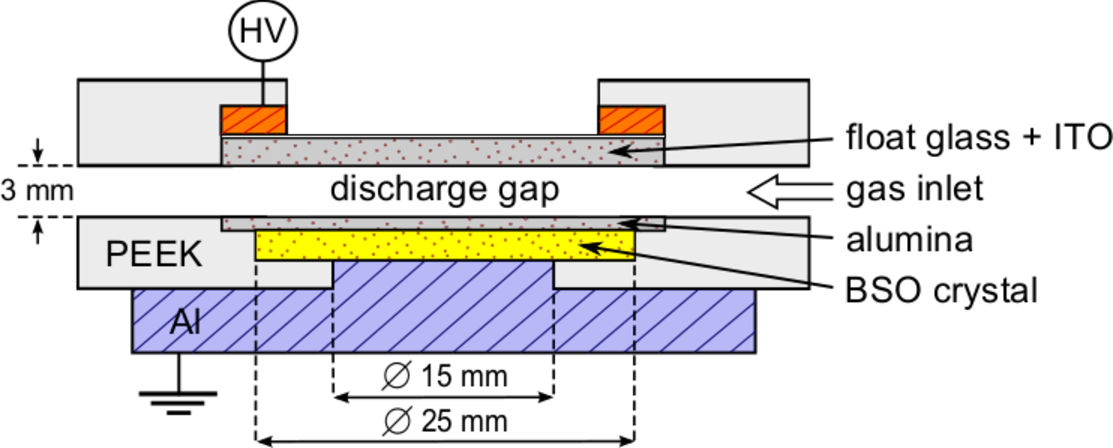
\includegraphics[width=0.5\textwidth]{figures/setup/discharge_cell.pdf}
					\caption{side-view of the concentric discharge cell. The variable dielectric was chosen to be mono-crystalline alumina.}
					\label{img:cell}
				\end{figure}
		
			The used discharge cell is sketched in \autoref{img:cell}. There, a symmetrical configuration, in which both plane, concentric electrodes are covered with dielectrics is shown. The gas gap width is $\unit[3]{mm}$ in height, whereas the diameter of the electrode is $\unit[15]{mm}$. A high-voltage driven copper ring is on top of a float glas plate, which is also covered with an electrically conductive, transparent indium tin oxide  (\tilt{ITO}) layer. On the bottom, a grounded aluminium mirror holds a bismuth silicon oxide (\tilt{BSO}) crystal. On top of that, a variable dielectric can be mounted, which is fixed to be aluminium in this experiment. Here, \tilt{mono-crystalline alumina} (Al$_2$O$_3$) was used. In advance for further investigations, it is crucial to know the different permittivities and dimensions of any used cell components - see \autoref{tab:permits}. The corresponding capacitance is calculated by $C\ix{x}=\varepsilon\ix{x}\varepsilon_0 A/2d$.\\
			The whole construct is mounted inside a steel vacuum chamber. A turbomolecular and process pump evacuate the chamber to a base pressure of about $\unit[\tenpo{-5}]{mbar}$, which ensures low concentration of impurities. Afterwards, the operating gas is passed from one side directly into the chamber through the polyetherethereton (\tilt{PEEK}) insulaters. Two mass flow controllers (MKS 647c) set the gas flow rate of Helium and Nitrogen (respective purity > 99,999\%) achieving high accuracy mixtures and flow rates of up to $\unit[100]{sccm}$. The discharge operated at elevated pressure levels of $\unit[1000]{mbar}$, which was kept constant through a diaphragm pressure gauge and butterfly valve (MKS) by the process pump (TRIVAC D25BCSPFPE).
			

				\begin{table}[h]
					\centering
					\begin{tabular}{c|c|c|c}
						material & d/mm & $\varepsilon\ix{r}$ & C/pF \\
						\hline glas+ITO & 0,7 & 7,6 & 169,88\\
						\hline Al$\ix{2}$O$\ix{3}$ & 0,2 & 10,55 & 825,36\\
						\hline BSO & 0,7 & 56 & 12,517 \\
					\end{tabular}
					\caption{Physical quantities of dielectrics inside discharge cell.}
					\label{tab:permits}
				\end{table}

		\subsection{Electrical diagnostics}\label{subsec:electric}
		
				\begin{figure}
					\centering
					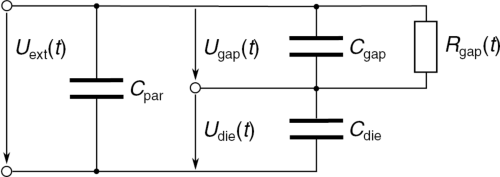
\includegraphics[width=0.5\textwidth]{figures/setup/replacementcircuit}
					\caption{Electrical equivalent circuit: the discharge gap is represented by the time-dependent resistance $R\ix{gap}(t)$ and $C\ix{gap}$ in parallel.}
					\label{img:circuit}
				\end{figure}
		
					 
			 As shown in \autoref{img:diag}, a function generator (SRS DS345) provides the voltage signal for the upper electrode, which ignites the discharge after its been amplified by a factor of 1000 (Trek 615-10), at a frequency of $\unit[5]{kHz}$ and amplitude of $\unit[1,2]{kV}$. The voltage can be a sine or square wave, dominating the discharge modes.\\
			 Applied voltage $U\ix{app}(t)$ and total transported charge $Q\ix{ext}$ are measured via a HV probe of 1000:1 and an external capacitor as well as a resistor, $C\ix{ext}=\unit[1]{nF}$ and $R\ix{ext}=\unit[100]{\Omega}$. The collection of data itself is utilized by a digital oscilloscope (ROHDE\&SCHWARZ RTO1024) with a bandwidth of $\unit[2]{GHz}$, which is connected through ethernet ports to a PC, running a customized LabView VI. Additionally, a Rogowski coil is attached to the cell, accumulating the flowing current and providing a much faster and higher slope. This will also be used as the trigger for the oscilloscope.\\
			 Furthermore, by using Lissajous figures $Q(U)$, one gains access to the breakdown charge $\Delta Q$ and the determination of the total capacitance of the discharge cell $C\ix{tot}$. By that, the gap voltage between the dielectrics $U\ix{gap}$ and the discharge current $I\ix{dis}$ can be calculated. A replacement circuit can be constructed, as depicted in \autoref{img:circuit}. Here, $C\ix{die}$ and $C\ix{gap}$ denote the dielectrics and discharge gap capacitance, taking into account the geometry. The parallel capacitance $C\ix{par}=C\ix{tot}-C\ix{gap}C\ix{die}/\left(C\ix{gap}-C\ix{die}\right)$ comprehends any volume in the cell not ignited by the discharge.\\
			 For this discharge configuration, it was calculated that $C\ix{BD}=\unit[500,92]{fF}$ and $C\ix{die}=\unit[12,66]{pF}$. Finally, one yields \cite{Kogelschatz2003}:
			 
				\begin{align*}
					 &U\ix{gap}(t)=\left(1+\frac{C\ix{par}}{C\ix{die}}\right)U\ix{ext}(t)-\frac{Q\ix{ext}(t)}{C\ix{die}} \,\, , \\
					 &I\ix{dis}(t)=\left(1+\frac{C\ix{gap}}{C\ix{die}}\right)\left(\frac{\diff Q\ix{ext}(t)}{\diff t}-C\ix{tot}\frac{\diff U\ix{ext}(t)}{\diff t}\right) \,\, .
				\end{align*}	

		\subsection{Optical emission spectroscopy}\label{subsec:oes}
		
				\begin{figure}
					\centering
					\hspace{-0.5cm}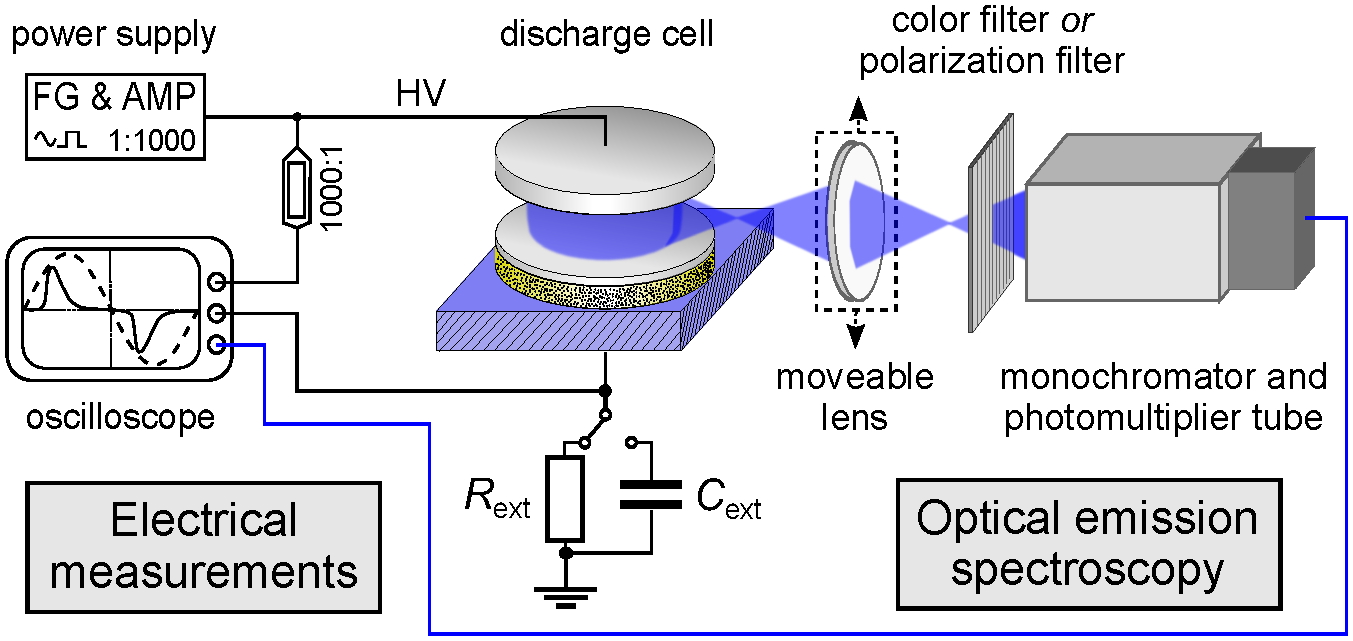
\includegraphics[width=0.5\textwidth]{figures/setup/setup}
					\caption{Set-up of the diagnostics used, with the corresponding discharge cell configuration.}
					\label{img:diag}
				\end{figure}
		
			The \autoref{img:diag} illustrates the diagnostic setup, by which the simultaneous investigation of electrical quantities, like charge and current, as well as the optical emission from the discharge is possible.\\		Here, the spatio-temporally resolved acquisition of single photons is accessible through a high-gain photomultiplier (\tilt{PM}: Becker\&Hickl PMH-100), a 1:1250 amplifier and monochromator. The fully movable optical system of two lenses, one slit and three vernier screws for vertical and horizontal adjustments across the full discharge cell, is focused via 1:-1 onto the monochromator (\tilt{MC}: Horiba, Triax 320). In this case, a spatial resolution of $\unit[0,1]{inch}$ or $\unit[0,15]{inch}$ is chosen. Through the combination of rogowski coil and digital oscilloscope a temporal resolution down to $\unit[2]{ns}$ is achieved. With a grating of $\unit[2400]{mm^{-1}}$, the monochromator achieves a spectral resolution of $\unit[0,02]{nm}$ at comparatively low intensities. At $\unit[1800]{mm^{-1}}$ one yields a lower resolution with higher photomultiplier currents.\\
			As the discharge frequency was chosen to be $\unit[5]{kHz}$, many data acquisitions per second can be performed by the digital oscilloscope. As the PM achieves a individually distinguishable electric signal for each photon, the raw data from the PM and amplifier has to be averaged over thousands of inner loops - for example 28000 averages at a sample rate of $\unit[100]{MSa/s}$ to cancel out any background noise. In addition, outer loops will be performed to rule out medium-range perturbations.\\
			For the line emission intensity ratio spectroscopy, the monochromator first scans a full spectrum between $\unit[585]{nm}$ and $\unit[730]{nm}$, including all Helium lines of interest. Specifically, those will be the already mentioned lines at $\unit[587,65]{nm}$, $\unit[706,66]{nm}$ triplet, as well as $\unit[728,31]{nm}$, $\unit[667.98]{nm}$ singlet. Surprisingly, those lines come with a small offset of $\approx\unit[0,15]{nm}$, compared to values obtained from various literature - see for example \href{http://www.nist.gov/pml/data/asd.cfm}{NIST Atomic Spectra Database} \cite{NIST_ASD}. This will be further discussed in the next section.\\
			While the line ratio measurement is based of a single wavelength, the Stark spectroscopy passes a small window of $\unit[0,7]{nm}$ in $\unit[0,02]{nm}$ steps. Therefore, the spectral resolution is much higher, whereas the intensity becomes smaller by many magnitudes.\\
			Both methods use the same setup, but differ in application. During the line emission spectroscopy, the optical system is elevated each time the measurement of all four lines is completed. Therefore, the entrance and exit slit of the MC are widened to $\unit[0,2]{mm}$ and vertically opened to $\unit[1]{mm}$. This way the cell gap is scanned with $\unit[0,05]{inch}$ steps.\\
			For Stark spectroscopy, the entrance/exit slit height is maxed out at $\unit[3]{mm}$, resulting in a lower spatial resolution of $\unit[0,1]{inch}$. Furthermore, the already mentioned polarization filter is placed along the optical axis between the MC and discharge cell.

	\section{Results}

		\subsection{Overview spectrum of optical emission}\label{subsec:overview}
		
			Here, the overview spectrum, which will be used for further investigations, is presented. The final results can be observed in \autoref{img:intspec}, which includes the indication of major peaks. Indeed those will be the target of the spatio-temporally resolved line emission spectroscopy in \autoref{subsec:stroe}.\\
			During the operation of this particular discharge, a mixture of $\unit[100]{sccm}$ helium and $\unit[0,05]{sccm}$ nitrogen, with a relative purity of $>99,999\%$ was used. Furthermore, the discharge was excited and ignited by a square wave of $\unit[5]{kHz}$ with an amplitude of $\unit[1,2]{kV}$. The cell was kept at a constant, atmospheric pressure of $\unit[1]{bar}$ by the mass flow controller. In addition, any optical components were configured to ensure the best results possible: a grating of $\unit[1800]{mm^{-1}}$ for high intensities, a PMT amplifier running at $\unit[1250]{V}$ to ensure adequate photon acquisition, a spectral resolution of $\unit[0,5]{nm}$ and a slit opening of $\unit[3]{mm}\times\unit[0,2]{mm}$.\\
			The full data, ranging from $\unit[585]{nm}$ to $\unit[730]{nm}$ was then corrected by an offset and integrated. Here, one used any emission - whereas there should be none - between $\unit[592]{nm}$ and $\unit[612]{nm}$ to calculate an average of the background noise. Afterwards, the 'new' spectrum was evaluated to be the 'old' - say raw - minus the offset. Remaining was an emission profile over time for each wavelength step, which happened to be 291. The integrated spectrum was received by applying the \tilt{explicit Euler method} (see \cite{Wiki:Euler}).\\
			As already pointed out, \autoref{img:intspec} contains the positions and quantum mechanical transition terms for any peaks of interest in further experiments. Primarily, those are found to be the dominant lines in our spectrum. Especially the transition between $2^3$P-$3^3$S carries the maximum intensity measured. In \autoref{subsec:oes} and \autoref{sec:intro} it is already sketched, what kind of optical line emissions are investigated and which physical processes is behind those. Mainly, the spectrum shows intensity peaks from excited states of helium in singlet or triplet states. To be more precise, $2^3$P$-3^3$D and $2^3$P$-3^3$S contribute to a triplet transition, whereas $2^1$P-$3^3$S and $2^3$P$-3^3$S originate from a singlet. As shown in, e.g. \cite{linratio1_14}, the excitation of named states is induced by impacting electrons, generated in regions of high electric field strength. Therefore, these electrons are non-thermal and hence correspond directly to the field strength and intensity of the given transitions. Furthermore, the intensities are also independent of local densities due to the equal influence of the electron numbers to all excitation states. One should note here, that in \cite{linratio1_14} (Ivkovi{\'c} et al.) also self-absorption, line broadening and Doppler effects are discussed to verify the results. This is not necessary here, as this work is based on the given implementations of the collisional-radiative model.
			
				\begin{figure}[t]
					\centering
					\hspace{-0.5cm}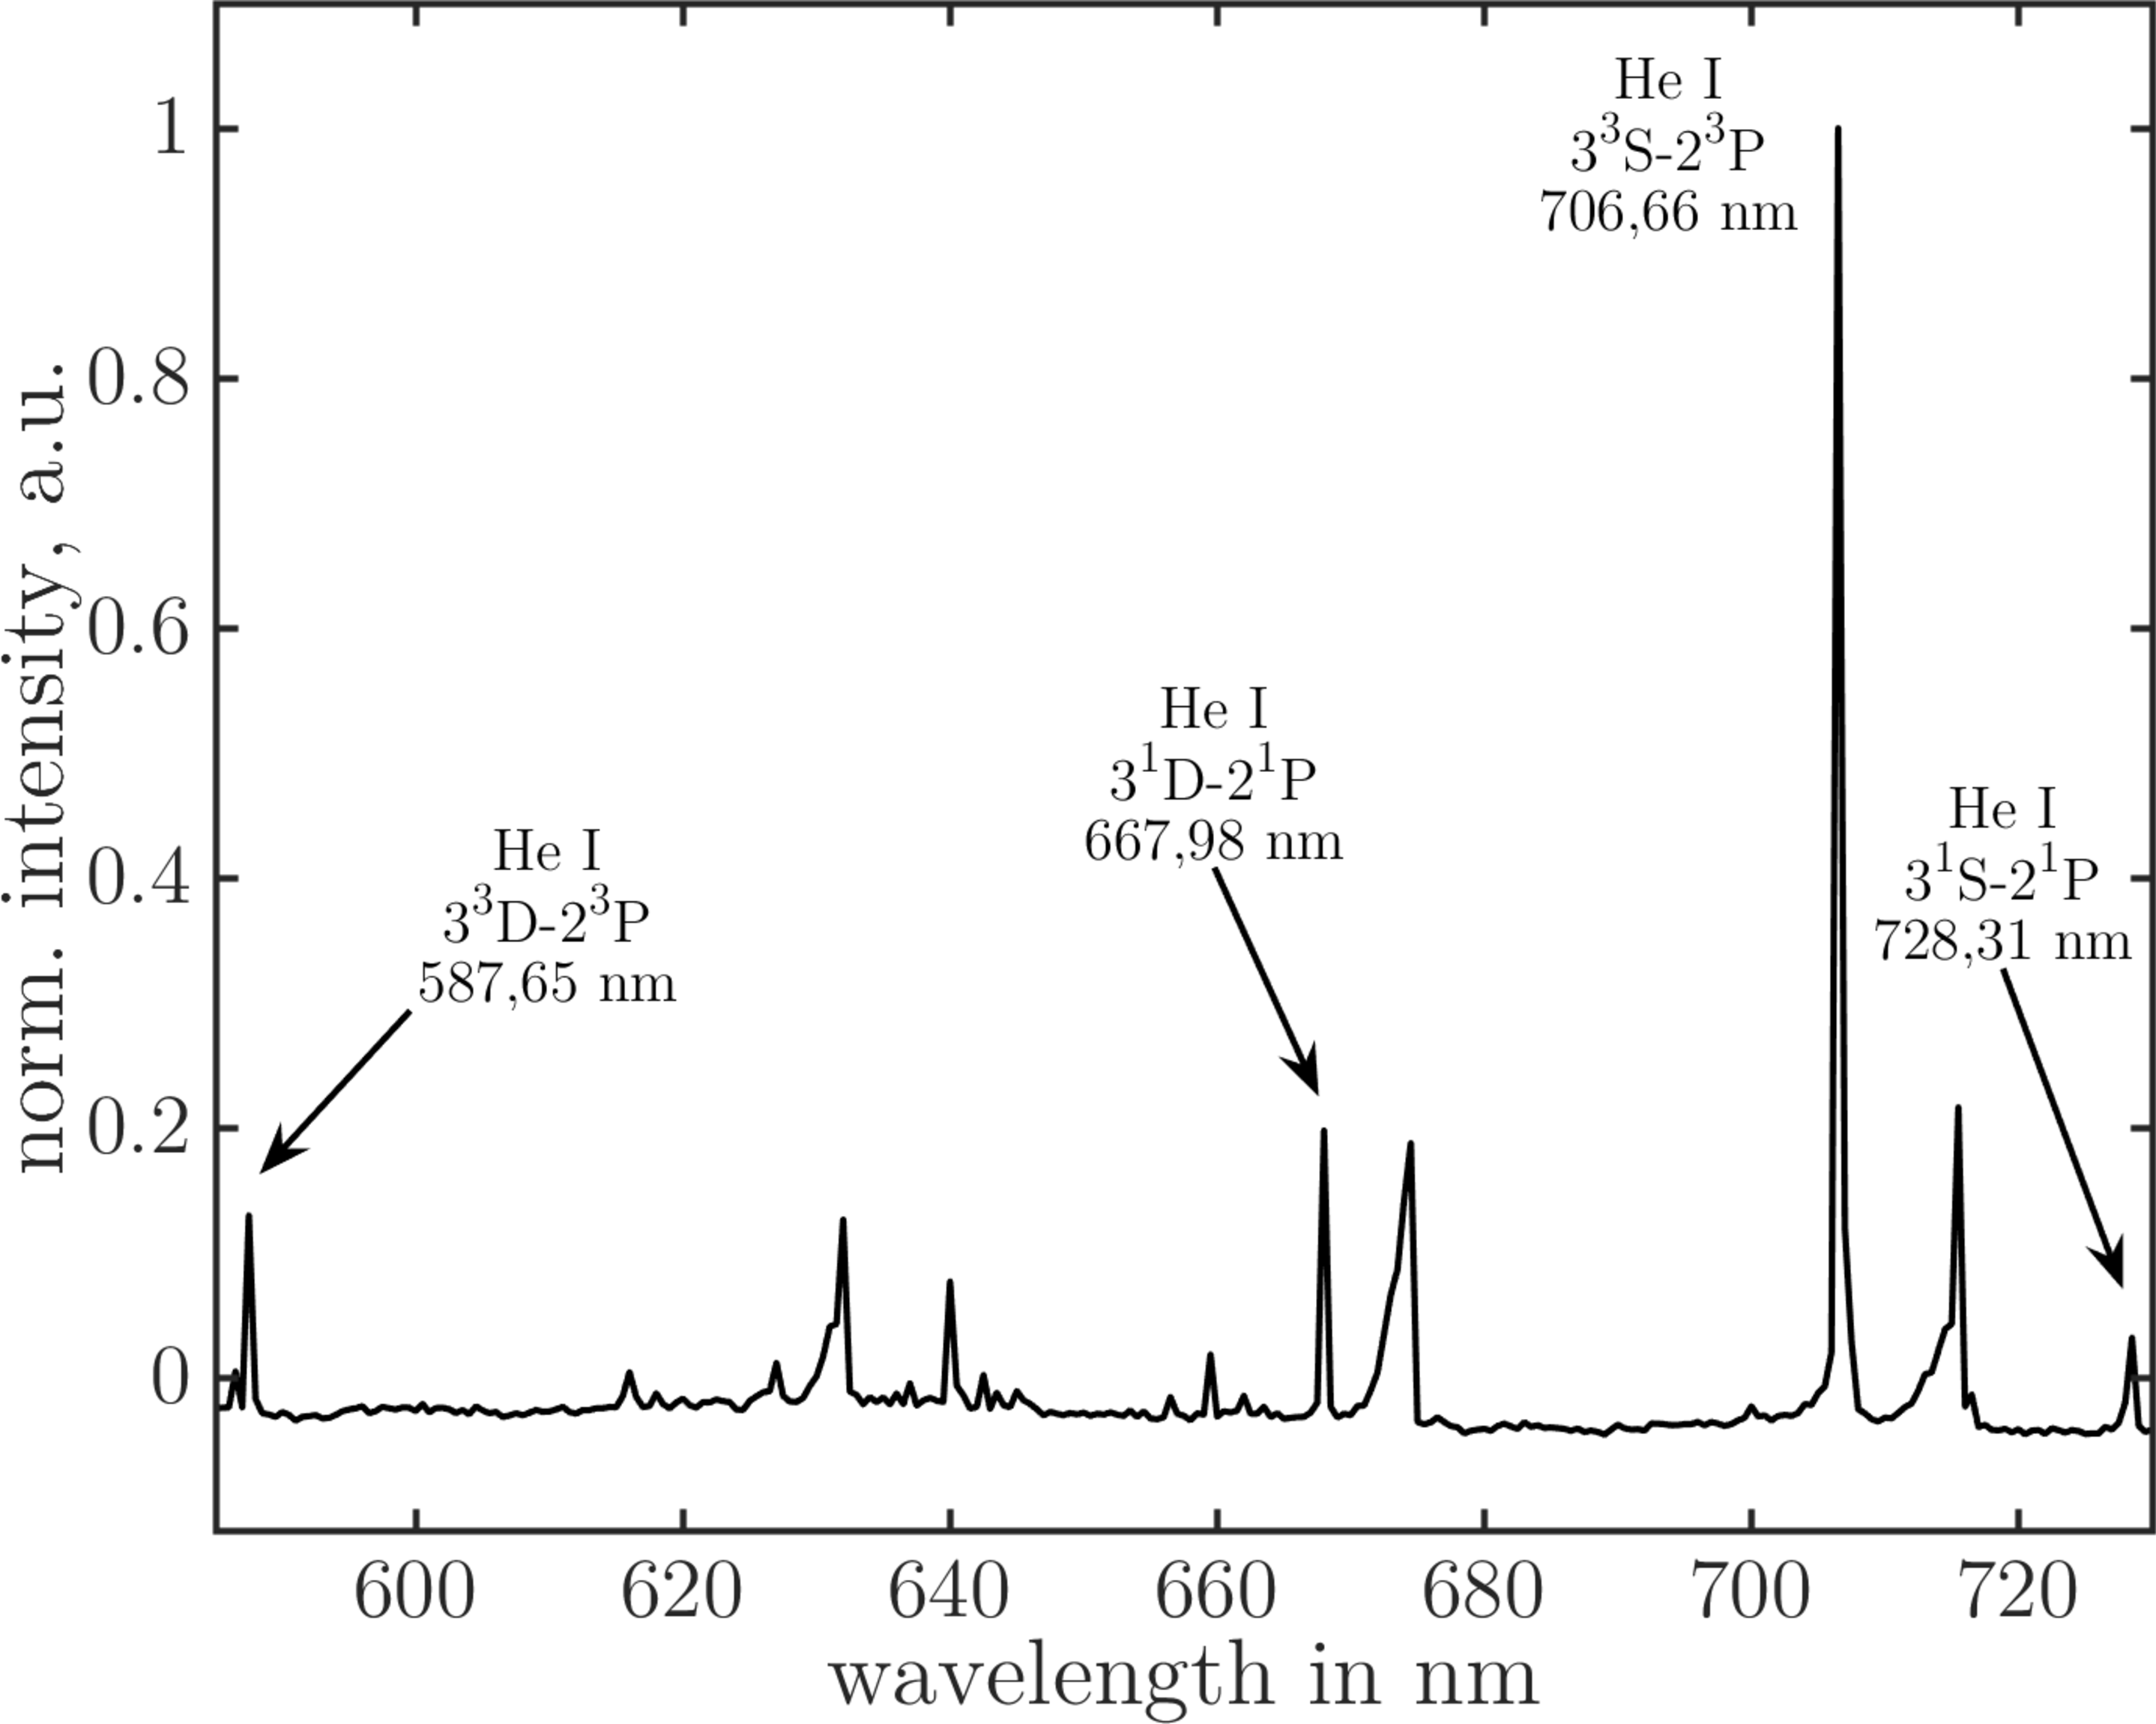
\includegraphics[width=0.5\textwidth]{figures/results/int_spectrum}
					\caption{Overview spectrum for a BD of $\unit[100]{sccm}$ He$_2$ and $\unit[0,05]{sccm}$ N$_2$ at a pressure of $\unit[1]{bar}$. Applied Voltage $\unit[1,2]{kV}$ at $\unit[5]{kHz}$.}
					\label{img:intspec}
				\end{figure}
			
			To get a more detailed look at the physical background, one has to look at the de-/ population of the named states as a result to electron impact. The ground and metastable level, $2^3$S and $2^3$S are much more significant in intensity than the spin forbidden counterpart $2^1$S. Also, transitions between 3P $\leftrightarrow$ 3D have been taken into account in following modelling. Depopulation is happening through spontaneous emission and associative ionization, which is common for atmospheric pressure BDs. Any electron induced depopulation is negligible. See \cite{PhysRevA.21.188}, \cite{0963-0252-14-4-011} for further investigations on cross sections and distribution functions.\\
			During low field strength phases of the discharge, excitation from metastable levels becomes more important. This is due to the low electron impact energy, which is then too low for excitation. Therefore, in any later evaluations one has to keep in mind, that the used model lacks a proper interpretation for low electric field strengths and the corresponding intensity in emission.\\
			Taking a look back at the full spectrum in \autoref{img:intspec}, one finds various additional peaks, than those already mentioned. This is due to the given mixture of He$_2$ and N$_2$ in the discharge cell. Minor impurities, like oxygen, hydrogen or carbon might contribute to this as well.\\
			Between $\unit[615]{nm}$ and $\unit[635]{nm}$, the second order of an emission band from OH can be found. Remaining H$\ix{2}$O molecules are dissociated by metastable helium atoms through penning ionization (see \cite{brandenburg2004raeumlich}). A rotation-vibrational emission band of molecular helium is ranging from $\unit[640]{nm}$ to $\unit[650]{nm}$. The final state of any contributing molecules is He$\ix{2}$(a$^{3}\Sigma\ix{u}$), a metastable, electronically excited dimer, and therefore influencing the population of our chosen triplet states. At $\unit[656]{nm}$, a line of the Pickering series - similar to the Balmer series of hydrogen - which corresponds to singly ionized He$^+$ (He I), is shown. Lastly, at around $\unit[675]{nm}$ and $\unit[718]{nm}$, the second order of both the SPS for N$\ix{2}$ (second positive system, N$\ix{2}$ II, 0-0 band) and lower shell transitions of He I, respectively, are peaking.
			
			%TODO DO I NEED THIS PARAGRAPH?!
			
			%Taking a look back at \autoref{img:intspec}, the full spectrum, one quickly finds many more peaks, with more or less intensity to them than the majoring transitions. This is due to the special mixture of He$_2$ and N$_2$ in the discharge cell - minor impurities might contribute to this as well. Here, a library for atomic spectra, the \href{http://physics.nist.gov/cgi-bin/ASD/lines1.pl}{NIST Atomic Spectra Database} was consulted. Without further reasoning, a short list of additional emission lines can be established (\autoref{tab:wavlg}). It should be sufficient here to only name those, because it will not be part of any profound considerations for following experiments.
		
		
		
				%\begin{table}
					%\centering
					%\begin{tabular}{l|c|c|r}
						%ion & term & lower level conf. & wavelength \\
						%\hline O IV & $^4$P & $2p^2(^3P)3s$ & $\unit[616,775]{nm}$ \\
						%\hline N II & $^3$F$^0$ & $2s{^2}2p3d$ & $\unit[617,331]{nm}$ \\
						%\hline C II & $^2$P$^0$ & $2s{^2}4p$ & $\unit[625,98]{nm}$ \\
						%\hline O I & $^3$P & $2s{^2}2p^4$ & $\unit[630,03]{nm}$ \\
						%\hline N II & $^3$D$^0$ & $2s{^2}2p3d$ & $\unit[631,88]{nm}$ \\
						%\hline N I & $^4$D$^0$ & $2s{^2}2p^{2}(^3P)3p$ & $\unit[639,84]{nm}$\\
									%& 			&					&  - $\unit[644,17]{nm}$ \\
						%\hline C II & $^2$S & $2s{^2}3s$ & $\unit[6658,288]{nm}$\\
						%\hline N II & $^1$P & $2s{^2}2p3p$ & $\unit[661,056]{nm}$\\
						%\hline C III & $^3$P$^0$ & $1s{^2}2p(^2P^0)3s$ & $\unit[674,438]{nm}$\\
					%\end{tabular}
					%\caption{List of additional transitions, their corresponding wavelengths and level configurations. One should note, that a full overview of all possible emission in the area of $\unit[(585-730)]{nm}$ is not economical and will not be discussed.}
					%\label{tab:wavlg}
				%\end{table}
		
		
		
		\subsection{Spatio-temporally resolved optical emission}\label{subsec:stroe}
		
			In this section, the previous obtained results from the overview spectrum and line emission scans for the already highlighted peaks at $\unit[587,65]{nm}$, $\unit[706,66]{nm}$, $\unit[728,31]{nm}$ and $\unit[667.98]{nm}$ will be processed. In particular, we will look at the emission for He I ($2^3$P$-3^3$S) triplet, to investigate different discharge modes and compare their properties in advance to understand the characteristic processes of a BD, e.g. ionization and field strength.

		\onecolumn
				
				\begin{figure}
					\centering
					\begin{subfigure}[t]{0.49\textwidth}
						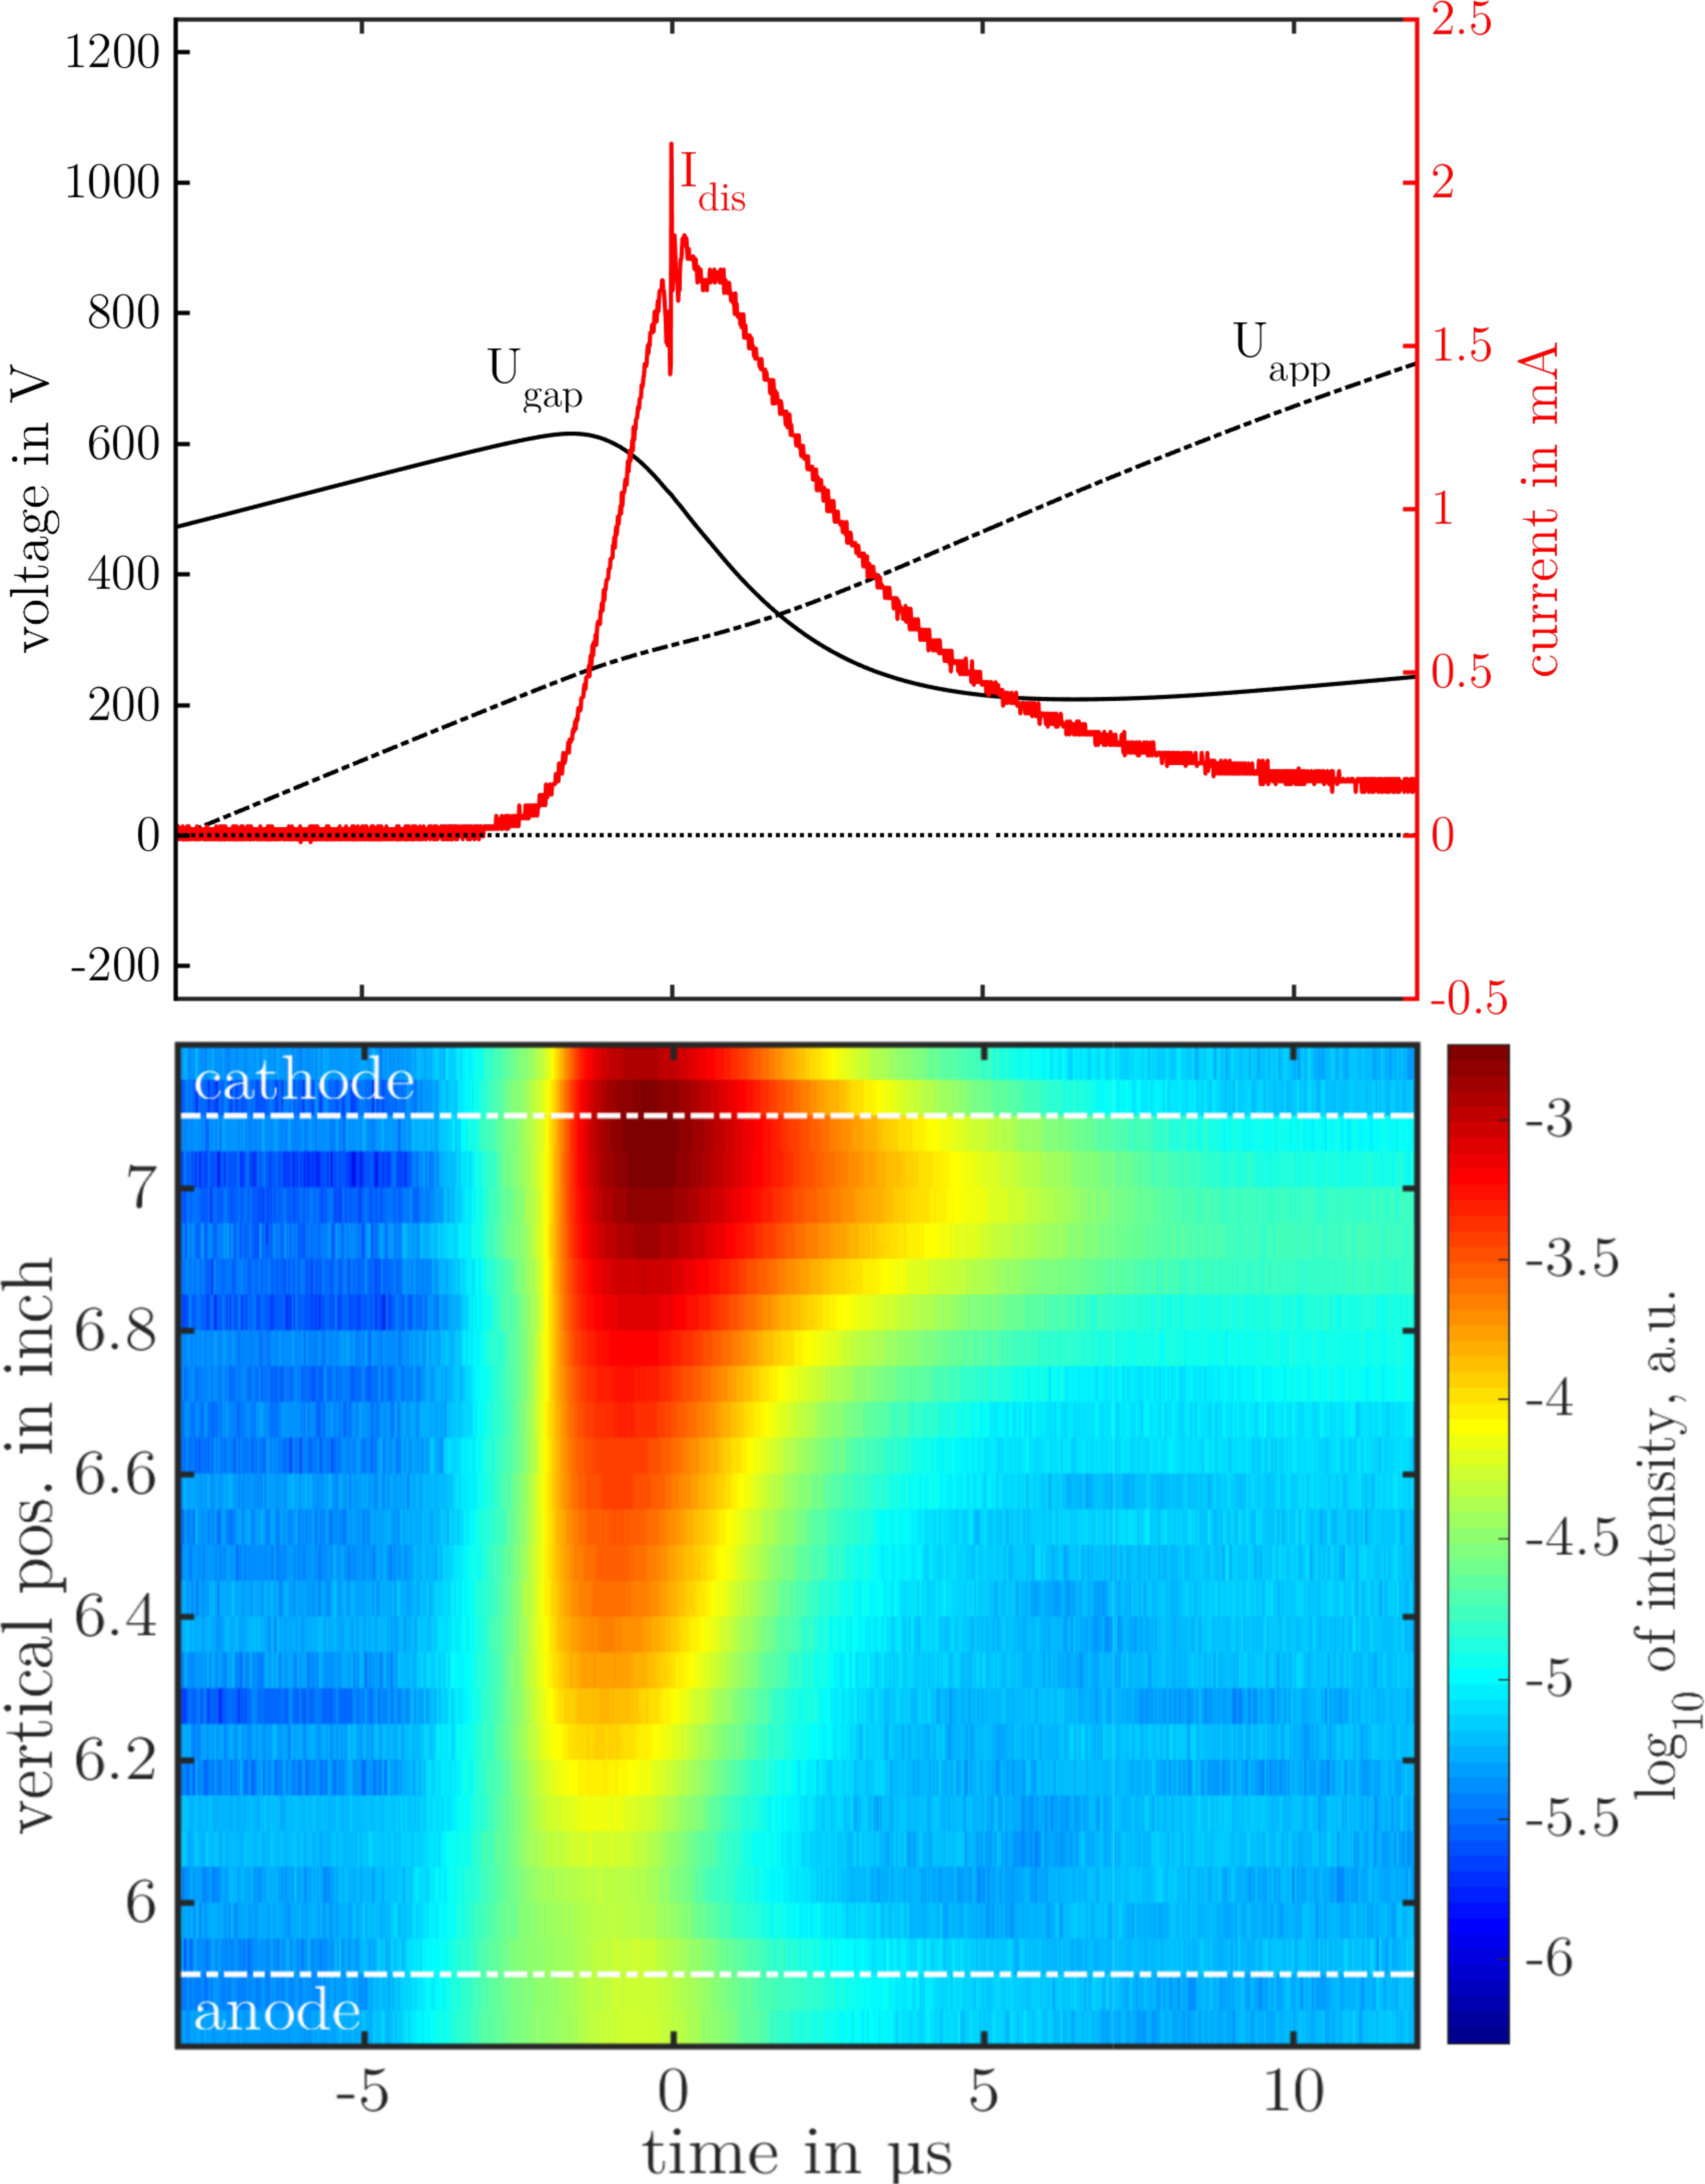
\includegraphics[width=\textwidth]{figures/706nm@sine/combination.pdf}
						\caption{}
						\label{img:combsine}
					\end{subfigure}
					\hfill
					\begin{subfigure}[t]{0.49\textwidth}
						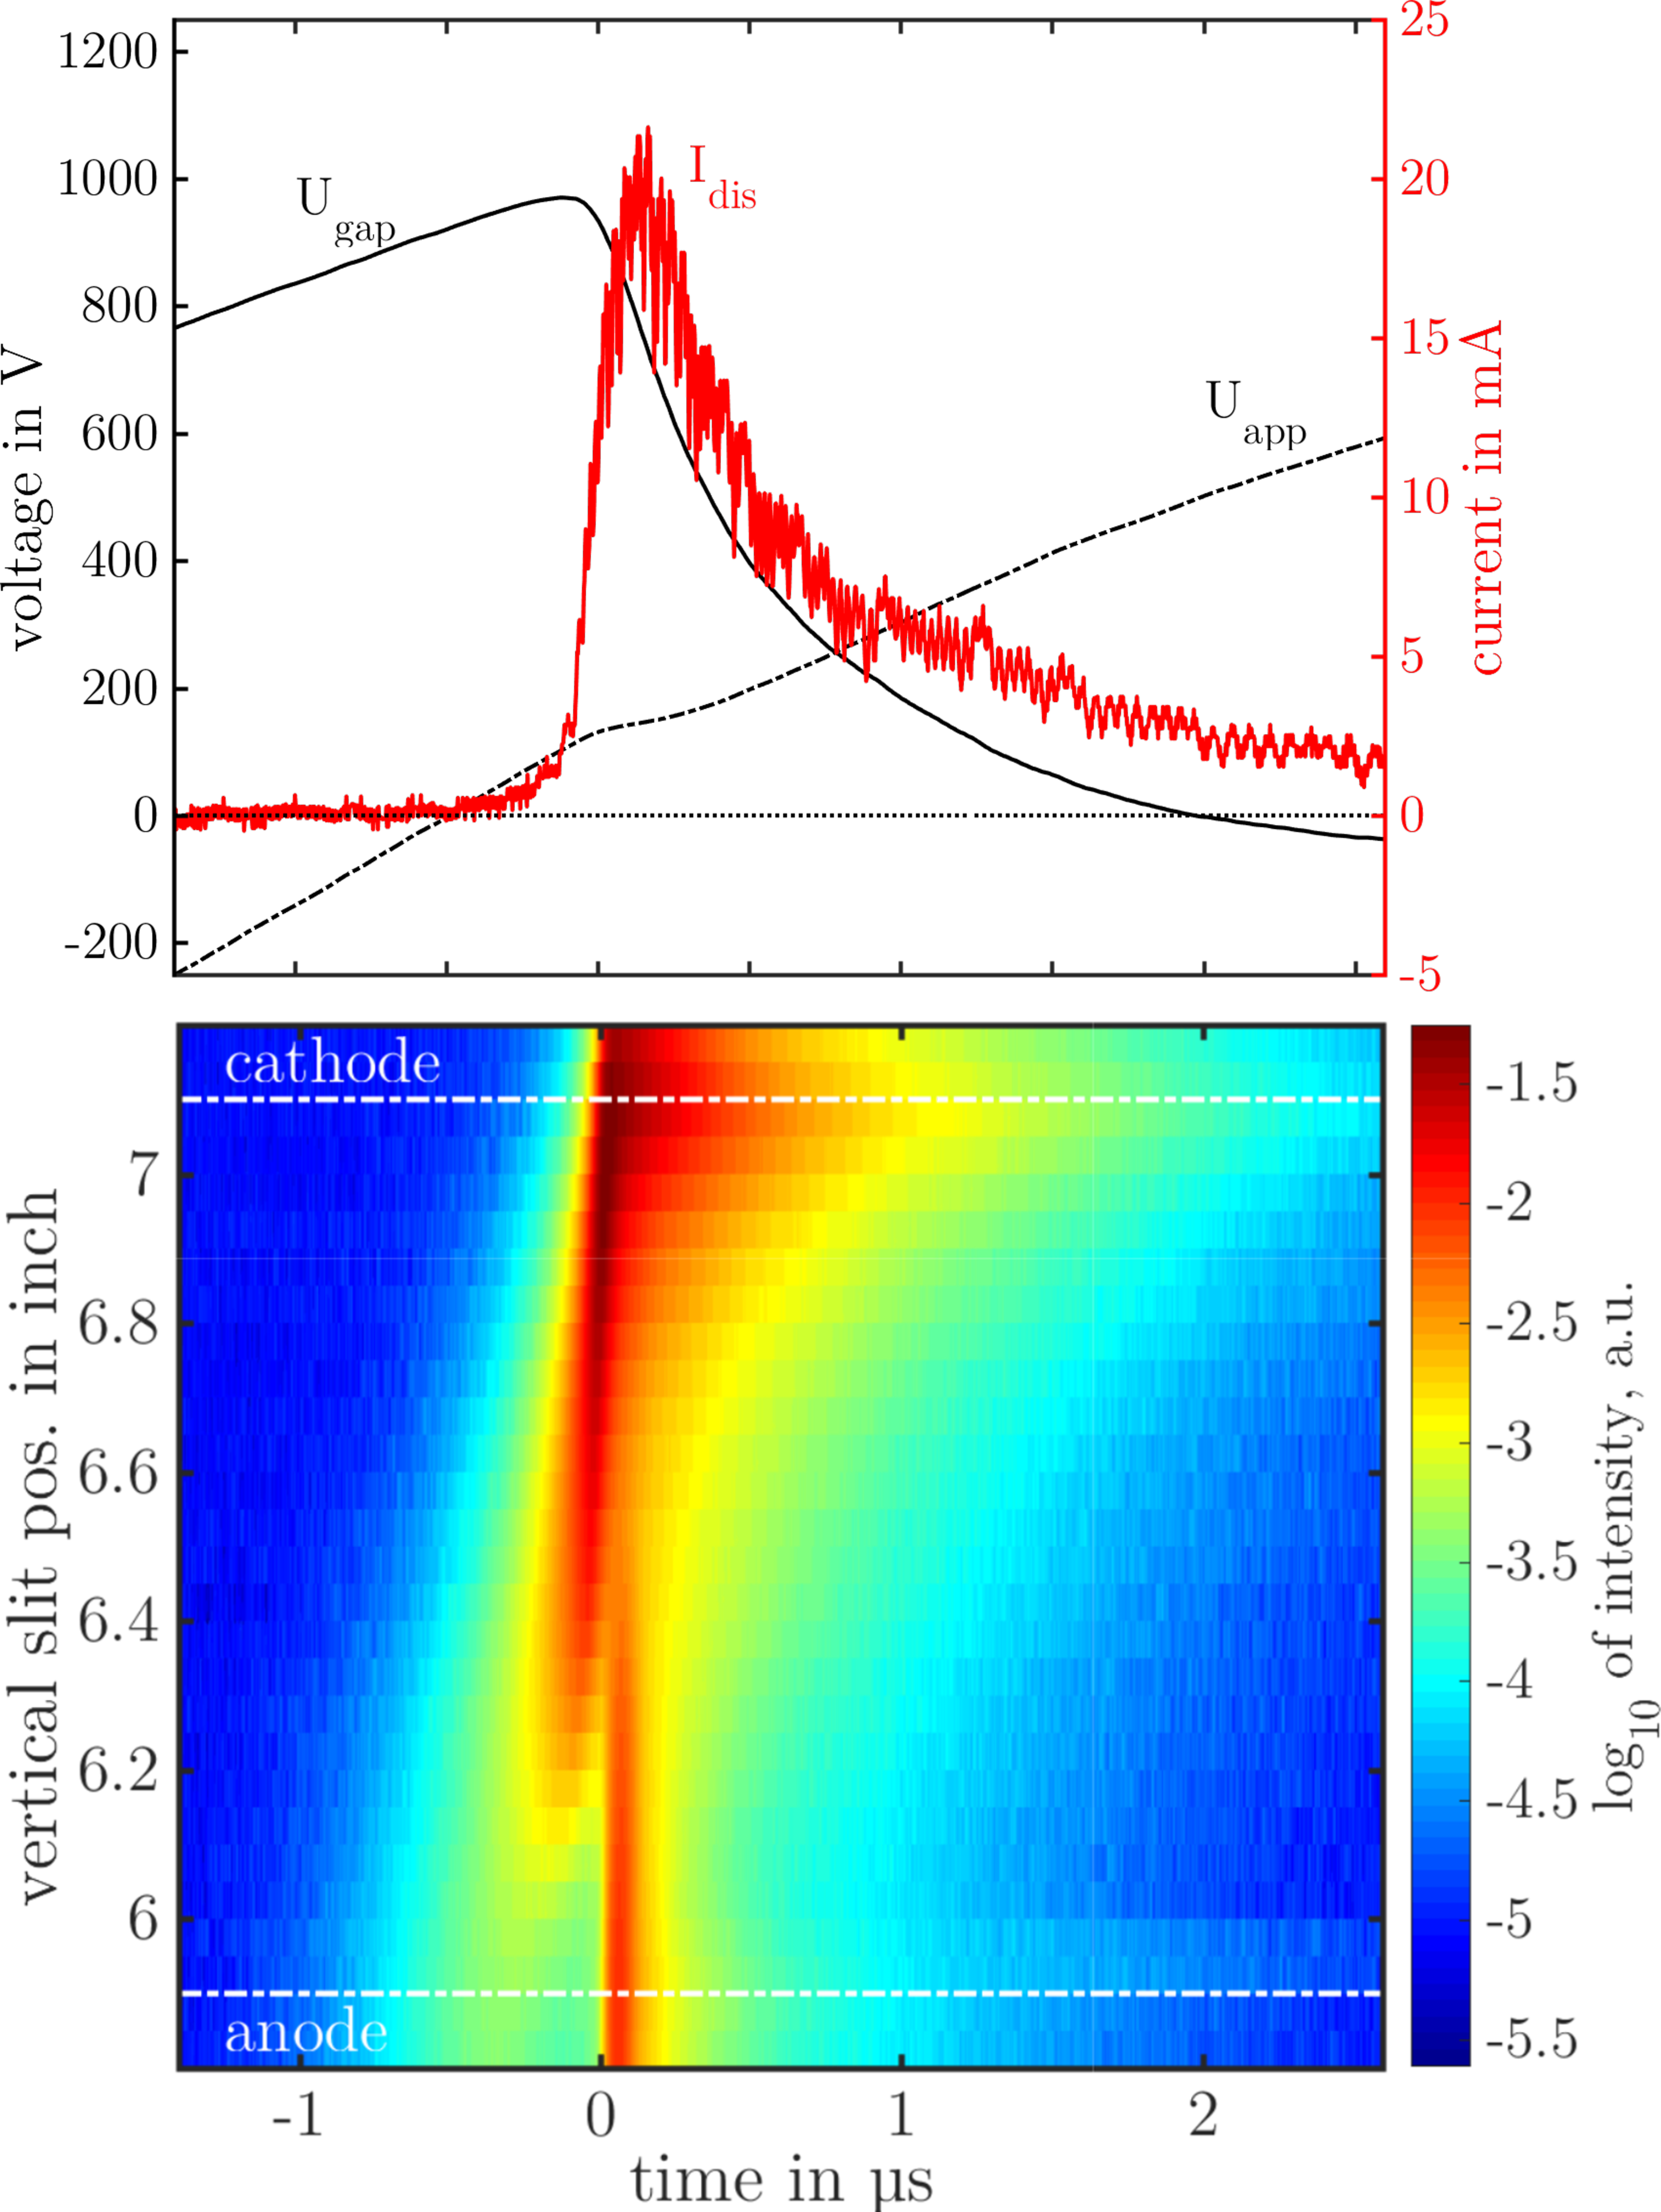
\includegraphics[width=\textwidth]{figures/706nm@square/combination.pdf}
						\caption{}
						\label{img:combsquare}
					\end{subfigure}
					\caption{Comparetive arrangement of spatio-temporally resolved emission profiles at $\unit[706,66]{nm}$ and discharge development for BDs excited by a \fett{(a)} sine, or \fett{(b)} square wave. For \fett{(a)} the properties were: $\unit[100]{sccm}$ He$_2$ + $\unit[0,05]{sccm}$ N$_2$ at $\unit[1]{bar}$\,; $\unit[1,2]{kV}$ at $\unit[5]{kHz}$ sine wave. In \fett{(b)}, only He$_2$ was used - at the same flow rate, voltage and frequency respectively. The excitation happened to be a square wave here.}
					\label{img:comparisonsinesquare}
				\end{figure}
				
			\begin{multicols}{2}
				Here, one will have a look at an comparative arrangement in \autoref{img:comparisonsinesquare} for discharges with applied voltages in sine (\autoref{img:combsine}) and square wave form (\autoref{img:combsquare}). Again, the flow rates for the square wave were $\unit[100]{sccm}$ He$_2$ and $\unit[0,05]{sccm}$ N$_2$ at $\unit[1]{bar}$\,, $\unit[1,2]{kV}$ at $\unit[5]{kHz}$ applied voltage and an equivalent optical setup properties to \autoref{subsec:overview}, despite that the vertical slit dimension now was $\unit[1]{mm}$ instead of $\unit[3]{mm}$. In the case of the sine wave,	only He$_2$ was used - at the same flow rate, voltage and frequency respectively. Additionally, an OG1 filter was put into the optical path to exclude unnecessary emissions from metastable nitrogen ions.\\
				For each of the mentioned wavelengths, a full vertical scan was done. That means, after an inner loop of 5 repetitions for a temporal measurement at a fixed height, the slit position was changed between $\unit[5,8]{inch}$ - the anode - and $\unit[7,2]{inch}$ - the cathode - with $\unit[0,05]{inch}$ steps. Therefore, the overall resolution calculates as $\unit[0,05]{inch}\times\unit[10]{ns}$.\\
				Data from the PMT were processed to result in \autoref{img:combsine} etc., by averaging over 5 loops and subtracting an offset measured at $\unit[690]{nm}$. Furthermore, the spectra are displayed logarithmic to emphasize gradients.\\
				First, we will take a closer look at the development of electrical properties of the discharges. As the top of \autoref{img:combsine} and \autoref{img:combsquare} are showing, both applied voltages $U\ix{app}$ have the same maximum, whereas their slope is different. Also, the gap voltage $U\ix{gap}$, which is the actual difference in electrostatic potential between anode and cathode (see \autoref{subsec:electric}), differs in amplitude and slope. Both show a collapse of $U\ix{gap}$ during the discharge breakdown, when the current $I\ix{dis}$ reaches its maximum. This is due to the transport of created charges inside the discharge volume onto the electrodes. They are accumulated on the dielectric surfaces, creating an opposing electric field. Therefore, the gap voltage drops sharply, which is why we are investigating a glow-like discharge mode. Here, strong ionization inside the discharge volume is found to cause significant currents of charges onto the dielectric surfaces. Hence, a greater negative slope in U$\ix{gap}$ during the breakdown implies increased ionization, and therefore a stronger discharge.\\
				In comparison to Townsend-like discharges, where the gap voltage remains constant during the breakdown, secondary electron emission is not significant. In APTDs, the discharge establishes an equilibrium current between charges from dielectric surfaces and volume, resulting in a less intense breakdown.\\
			\end{multicols}
				
		\twocolumn

			\begin{figure}
				\centering
				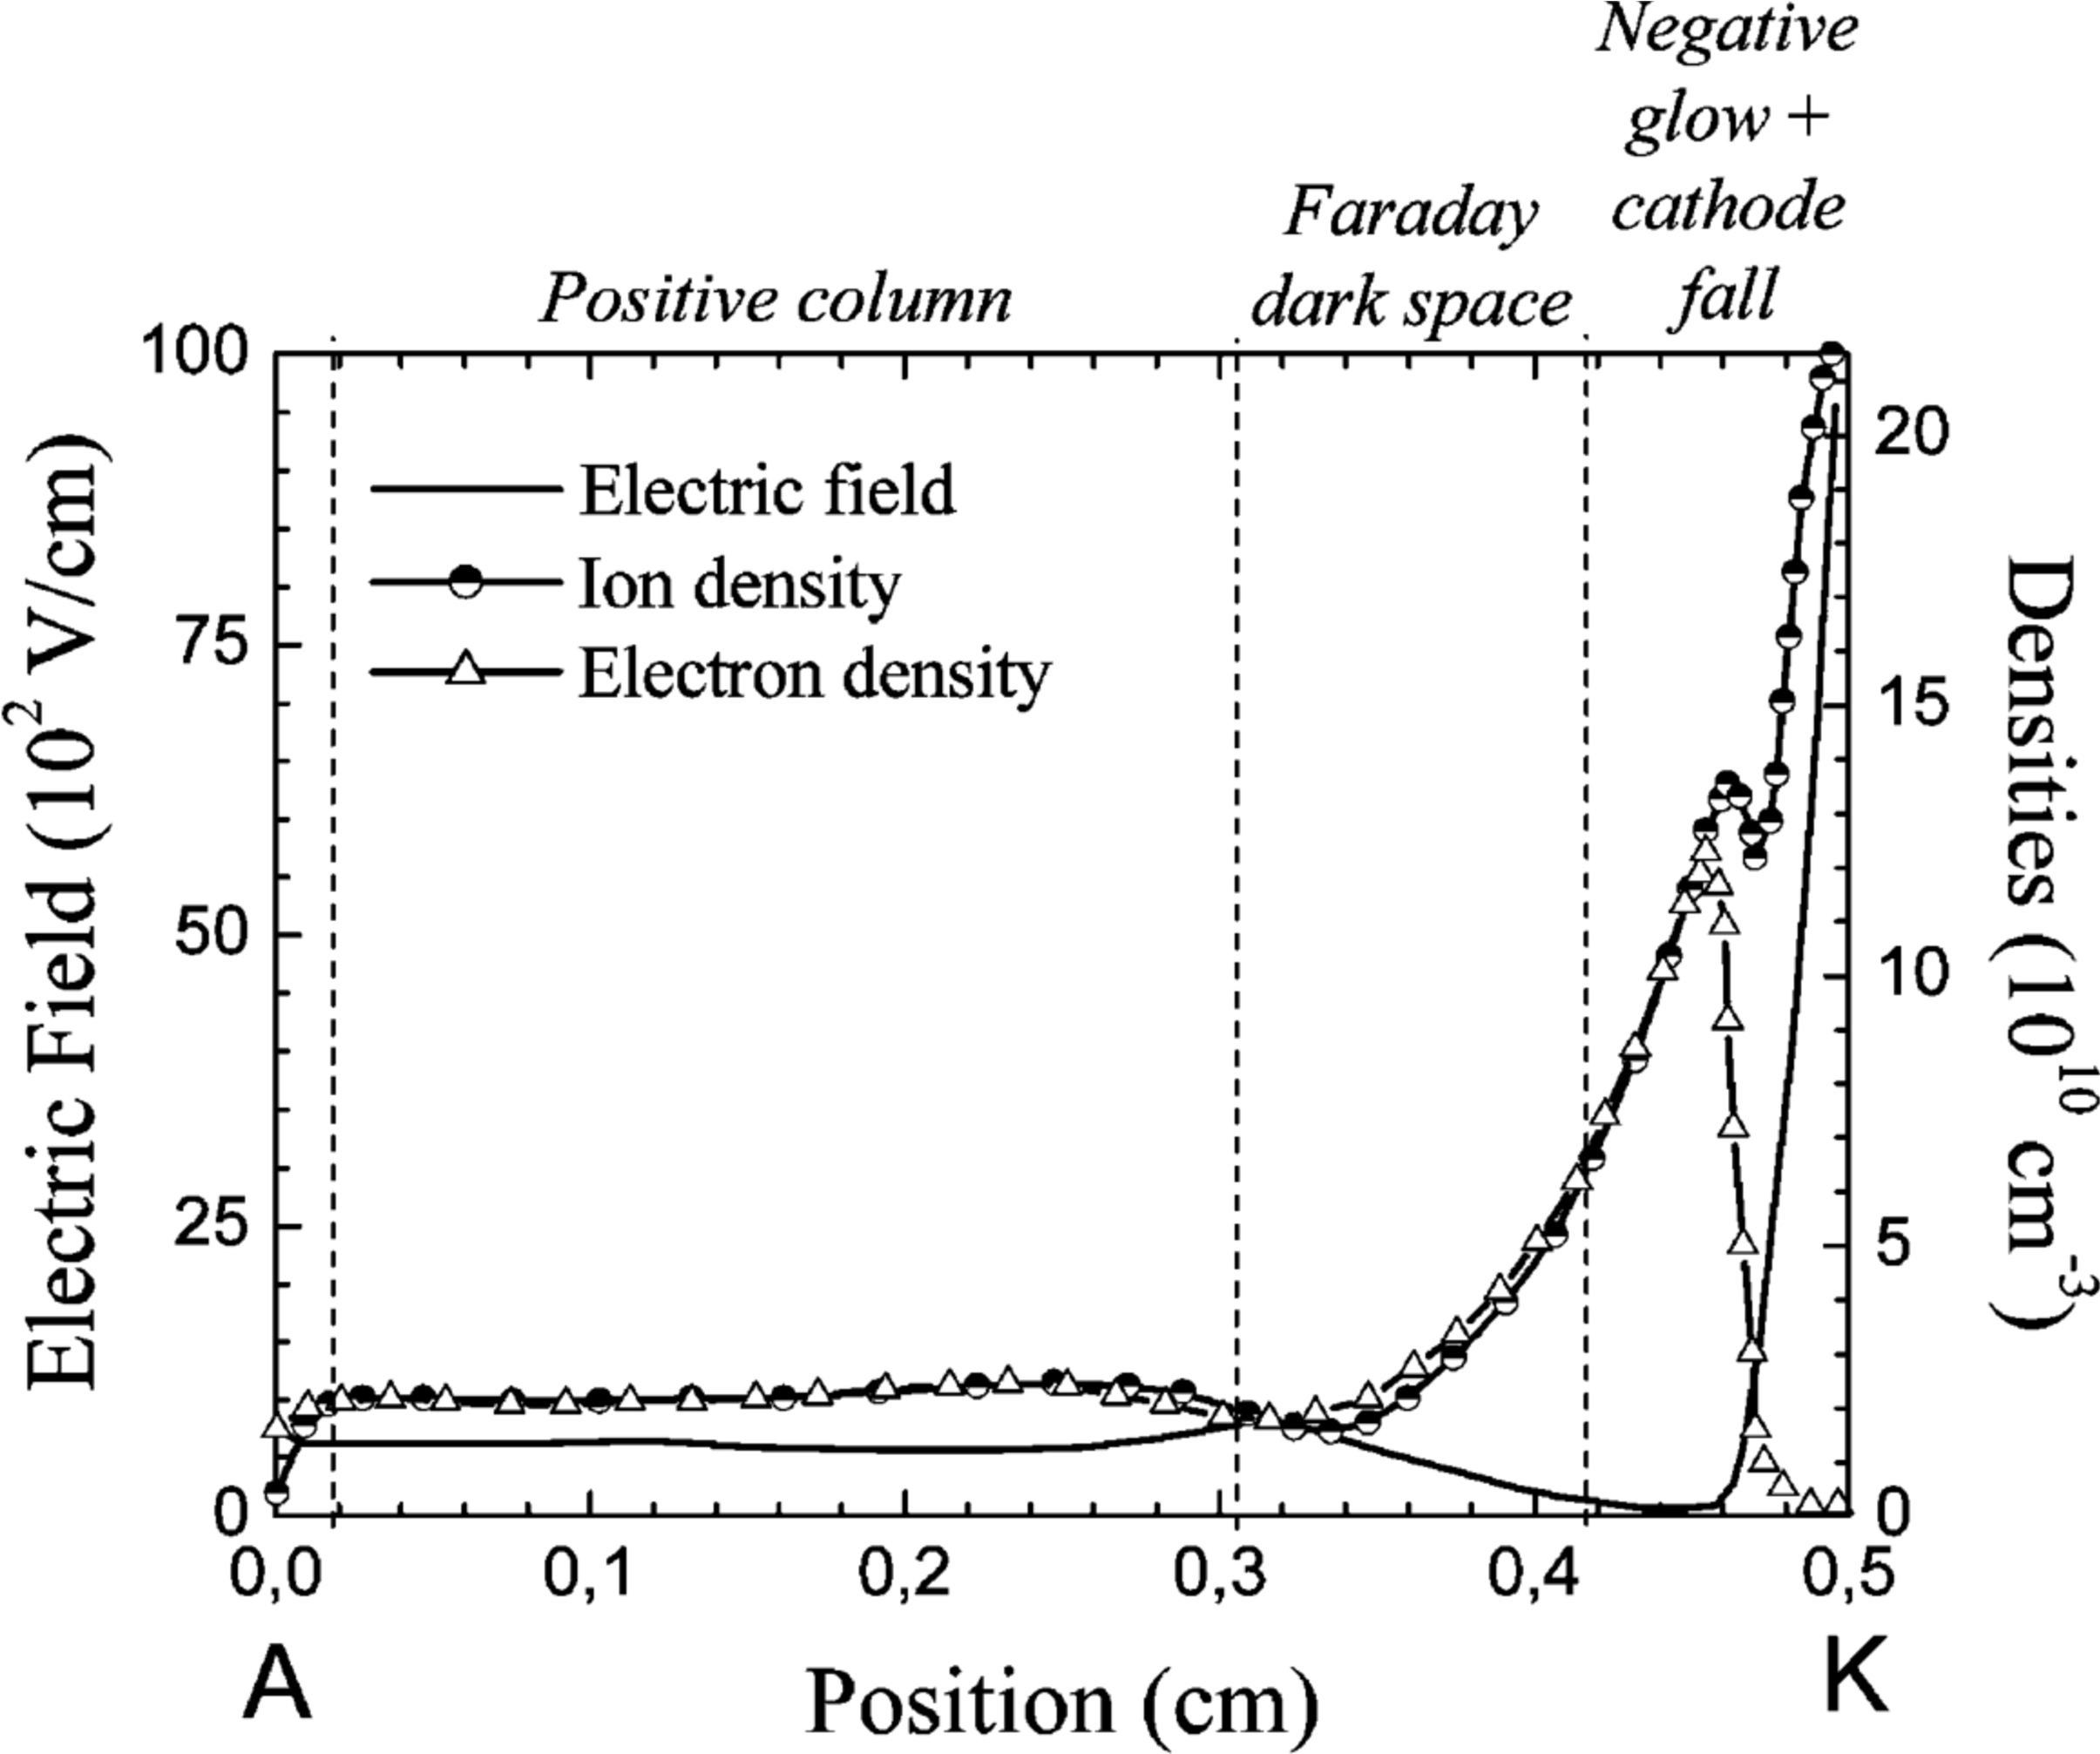
\includegraphics[width=0.5\textwidth]{figures/706nm@square/massinesp3fig5.pdf}
				\caption{Calculated space distribution from the anode to the cathode of	the electrical field, the ion and electron densities in a He glow dielectric barrier discharge when the discharge current intensity is maximum. \cite{Massines}}
				\label{img:massines}
			\end{figure}

		The discharge currents $I\ix{dis}$ also differ by one magnitude, as well as slope and width of the peak are not the same. This is due to a longer preliminary phase for an applied sinus wave voltage. A lower slope favors the accumulation of more volume charges, therefore attentuating the breakdown voltage even further. Furthermore, the sine wave has a longer rising time, which is why the observed current pulse is widened/lowered and the discharge less intense.\\					
		Now that the development of the electrical properties for our presented BDs and the different applied voltages has been evaluated, we will put those results in relation to the enclosed spatio-temporally resolved optical emission. The bottom of \autoref{img:combsine} and \autoref{img:combsquare} shows the temporal development of emission intensity at $\unit[706,66]{nm}$ between (dashed white lines) anode and cathode - see \autoref{img:golubovskii} for a theoreticaly calculated comparison. Above and beyond one can see a reflection from the dielectric surfaces.\\
		During the preliminary Townsend phase, both voltage forms show weak emission in front of the anode, which indicates the starting exponential electron multiplication. Therefore, positive space charges develop, as heavy ions are not as mobile as electrons in the accelerating, at this time nearly homogeneous electric field. The resulting cathode-directed ionization front culminates in the breakdown, right when the maximum current is flowing (see \autoref{img:massines}). Fast electrons are rushing towards the anode, exciting and ionizing on their path and therefore producing an increasing emission maximum towards the cathode. Behind this negative glow, there is space charge with almost no electrons. The ions are accelerated here, like in a gravitational free fall. This cathode fall region yields a very high electric field and high ion density.\\
		An anode-sided counterpart of the negative glow, which consists of a large space charge, is called positive column. This can only be seen at the emission profile of a square wave discharge. Only here, the ionization front moves quickly enough through the cell volume to develop the required current for a positive space charge.	Here, quasi neutrality is almost satisfied, which means the electric field strength is low and constant. Only shortly before the positive electrode, inside the anode dark space, electron and ion density decrease. Hence, the emission is attenuated there.\\
		Further on in the temporal development of the discharge, emission is decreasing as excited species are relaxing. The breakdown removes a majority of free charges, which is why flowing current and glow diminish over time. Here, the maximum remains in front of the cathode. This after glow is much wider and longer for a sine wave discharge, than for the square wave. This is due to the lesser slope in current, voltage and therefore slower charge transportation over the discharge volume.\\
		In \autoref{img:golubovskii} and \autoref{img:massines} theoretical calculated field strength developments over time and space are shown (\cite{Massines}, \cite{0022-3727-36-1-306}.) They greatly underline the findings of the previous section. Overall, the physical properties of interest may now be better understood with respect to temporal and spatial development. The key finding here should be the direct link between line emission of the singlet lines and the corresponding electric field strength.
		
			\begin{figure}
				\centering
				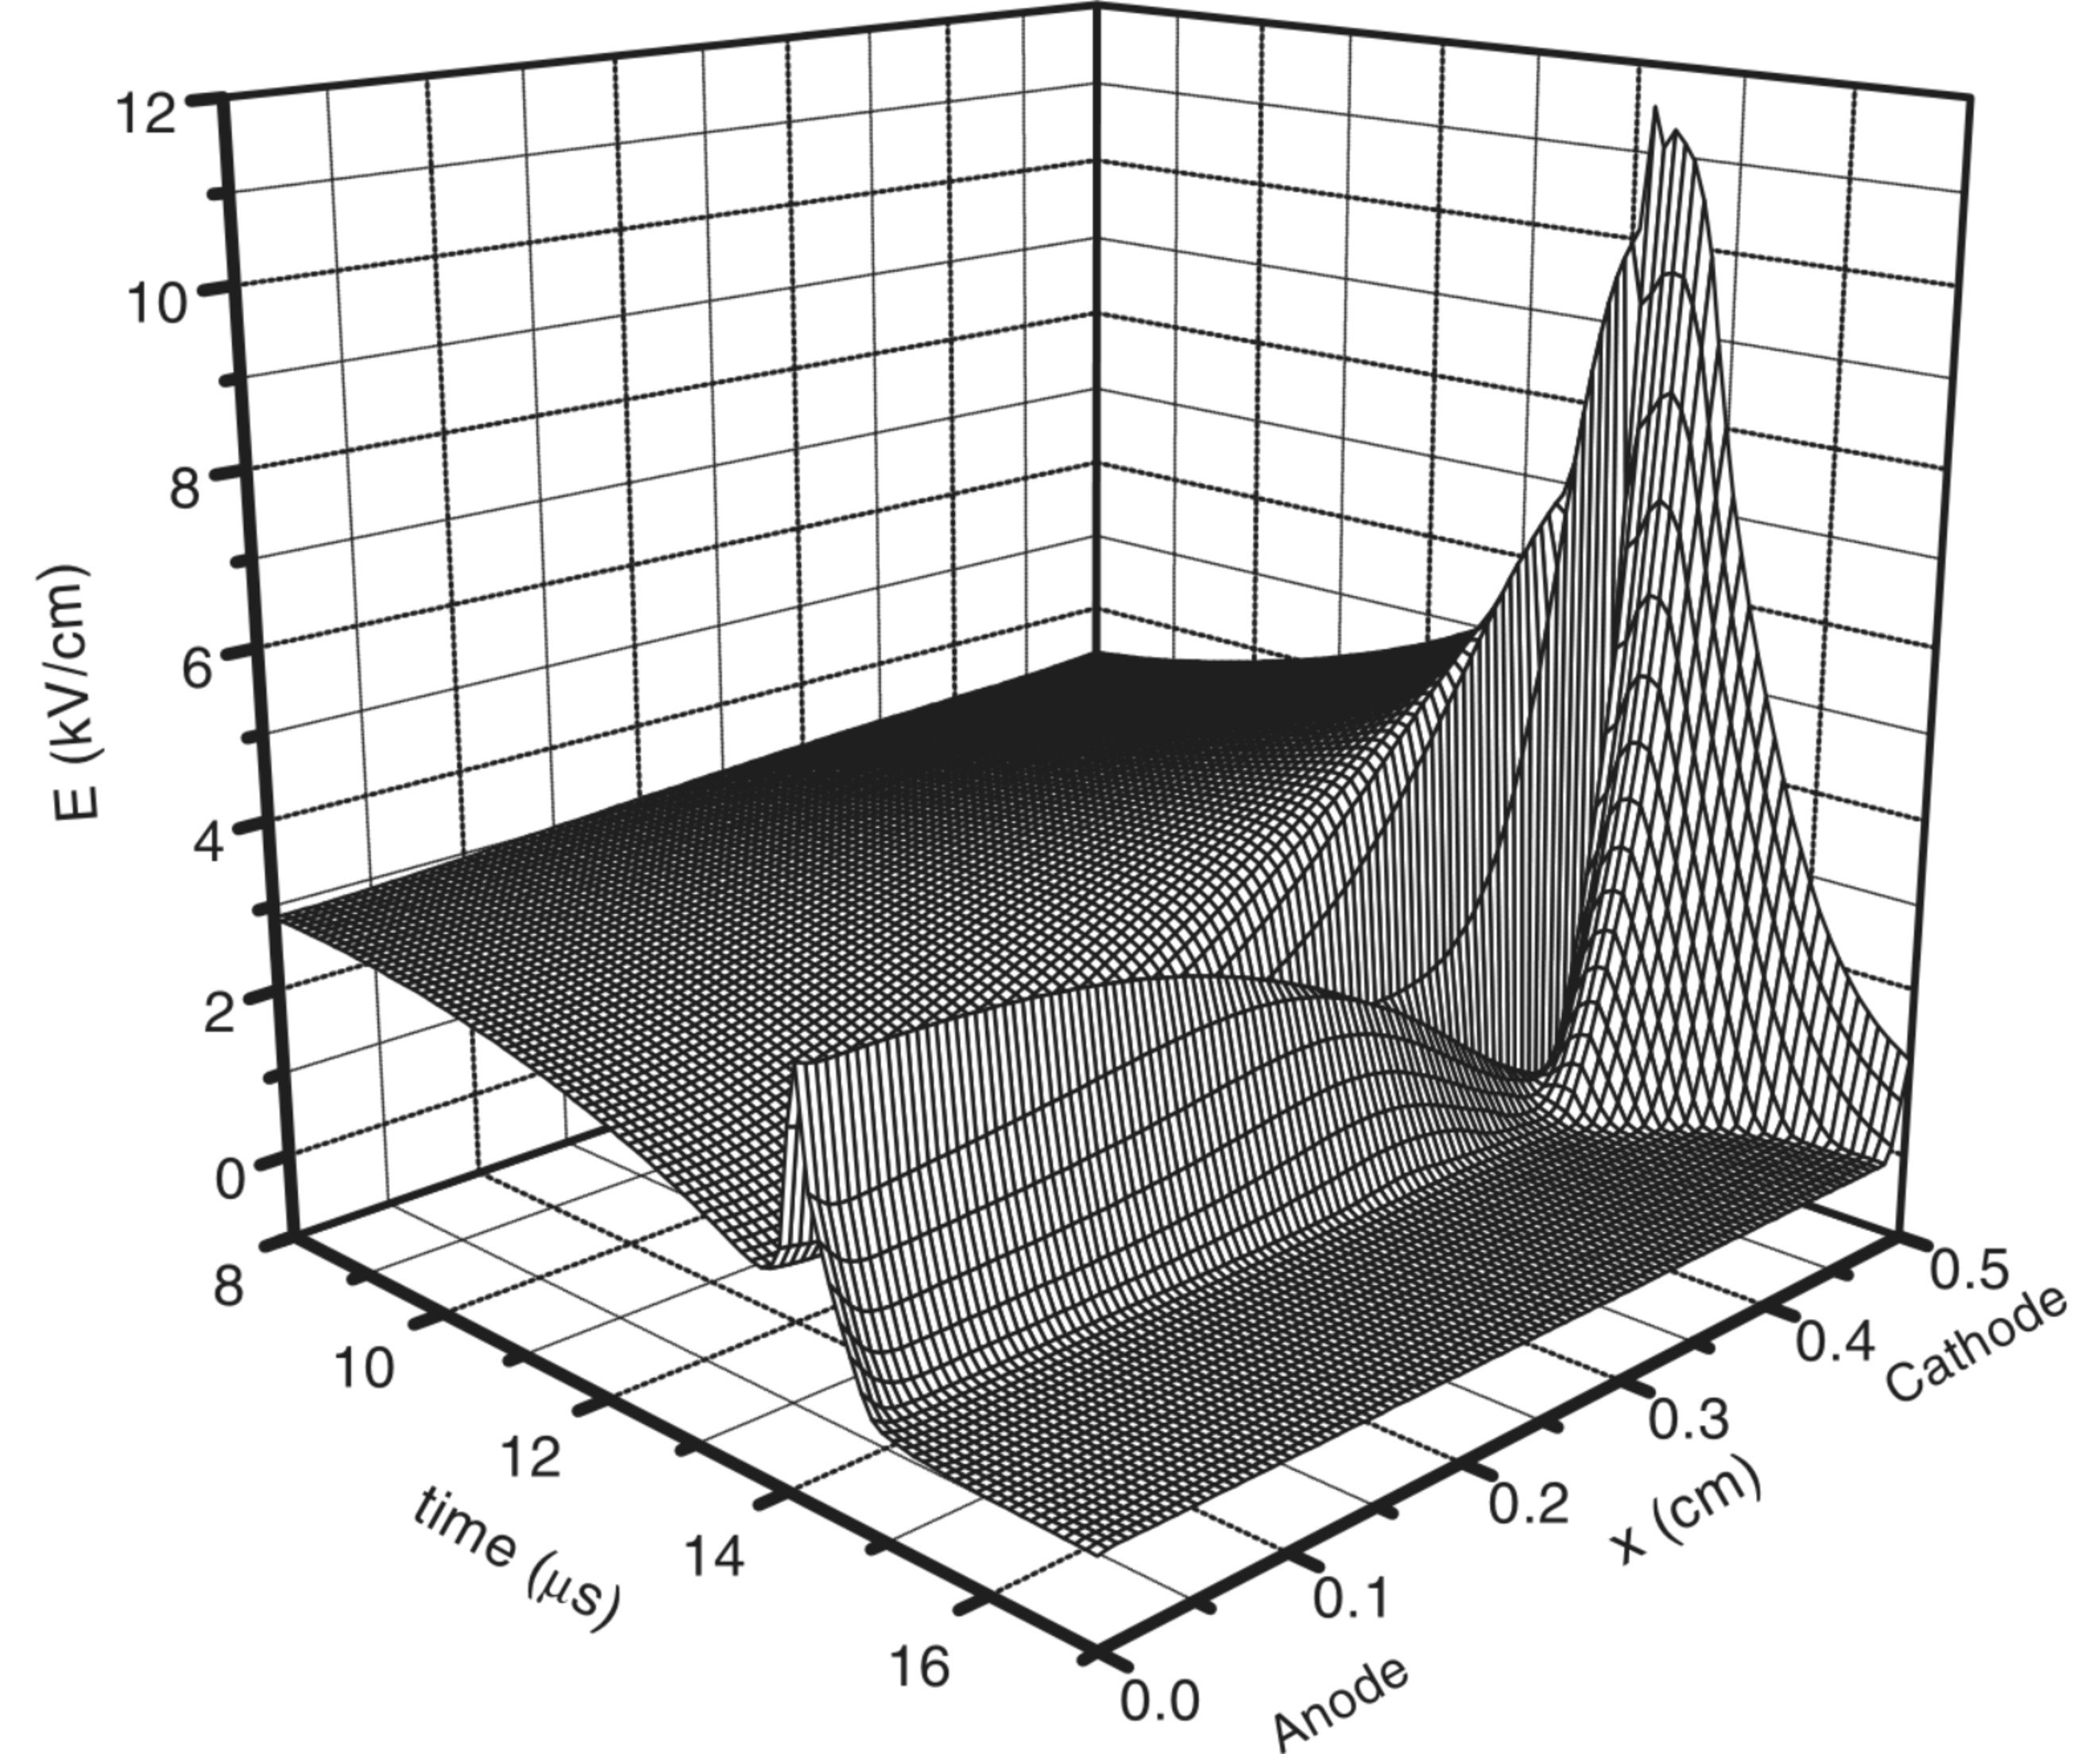
\includegraphics[width=0.5\textwidth]{figures/706nm@square/golubovskiip47fig9}
				\caption{Three-dimensional plot of the electric field strength in the breakdown phase of glow discharge. \cite{0022-3727-36-1-306}}
				\label{img:golubovskii}
			\end{figure}
		
			\onecolumn
			
			\begin{figure}
				\centering
				\begin{subfigure}[t]{0.49\textwidth}
					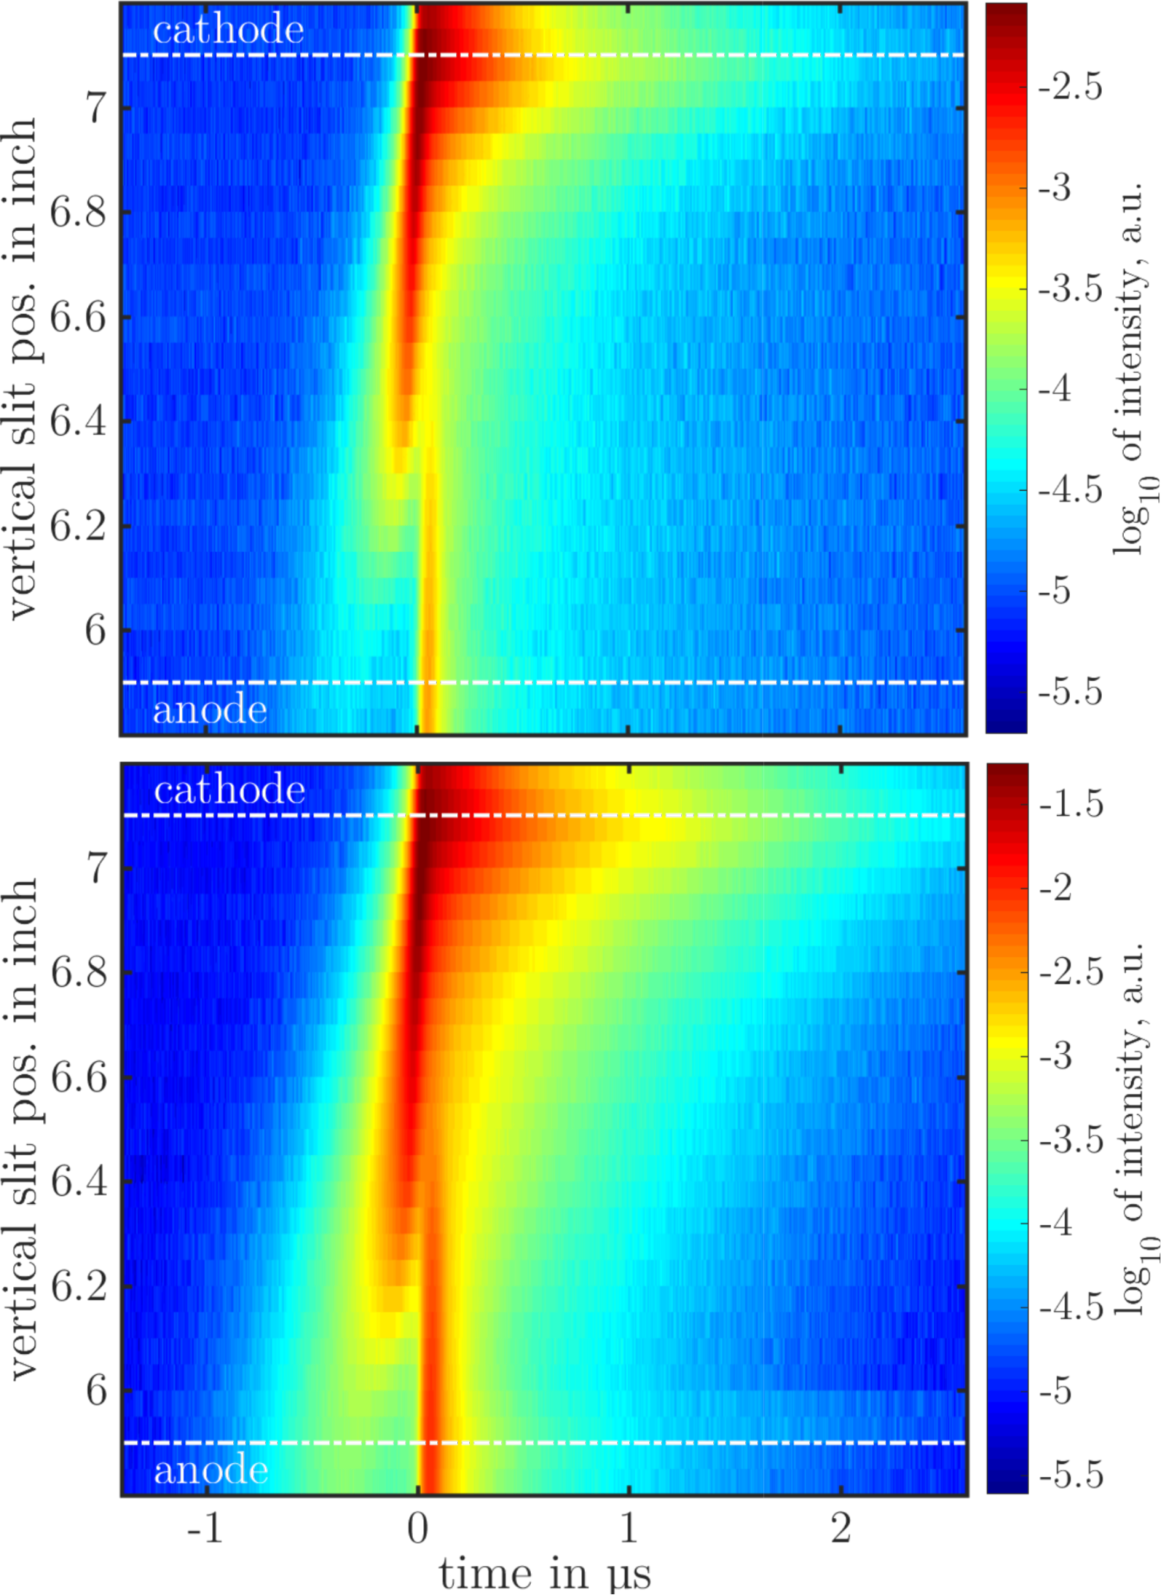
\includegraphics[width=\textwidth]{figures/lineratio/667u706.pdf}
					\caption*{}
					\label{img:667u706nm}
				\end{subfigure}
				\hfill
				\begin{subfigure}[t]{0.49\textwidth}
					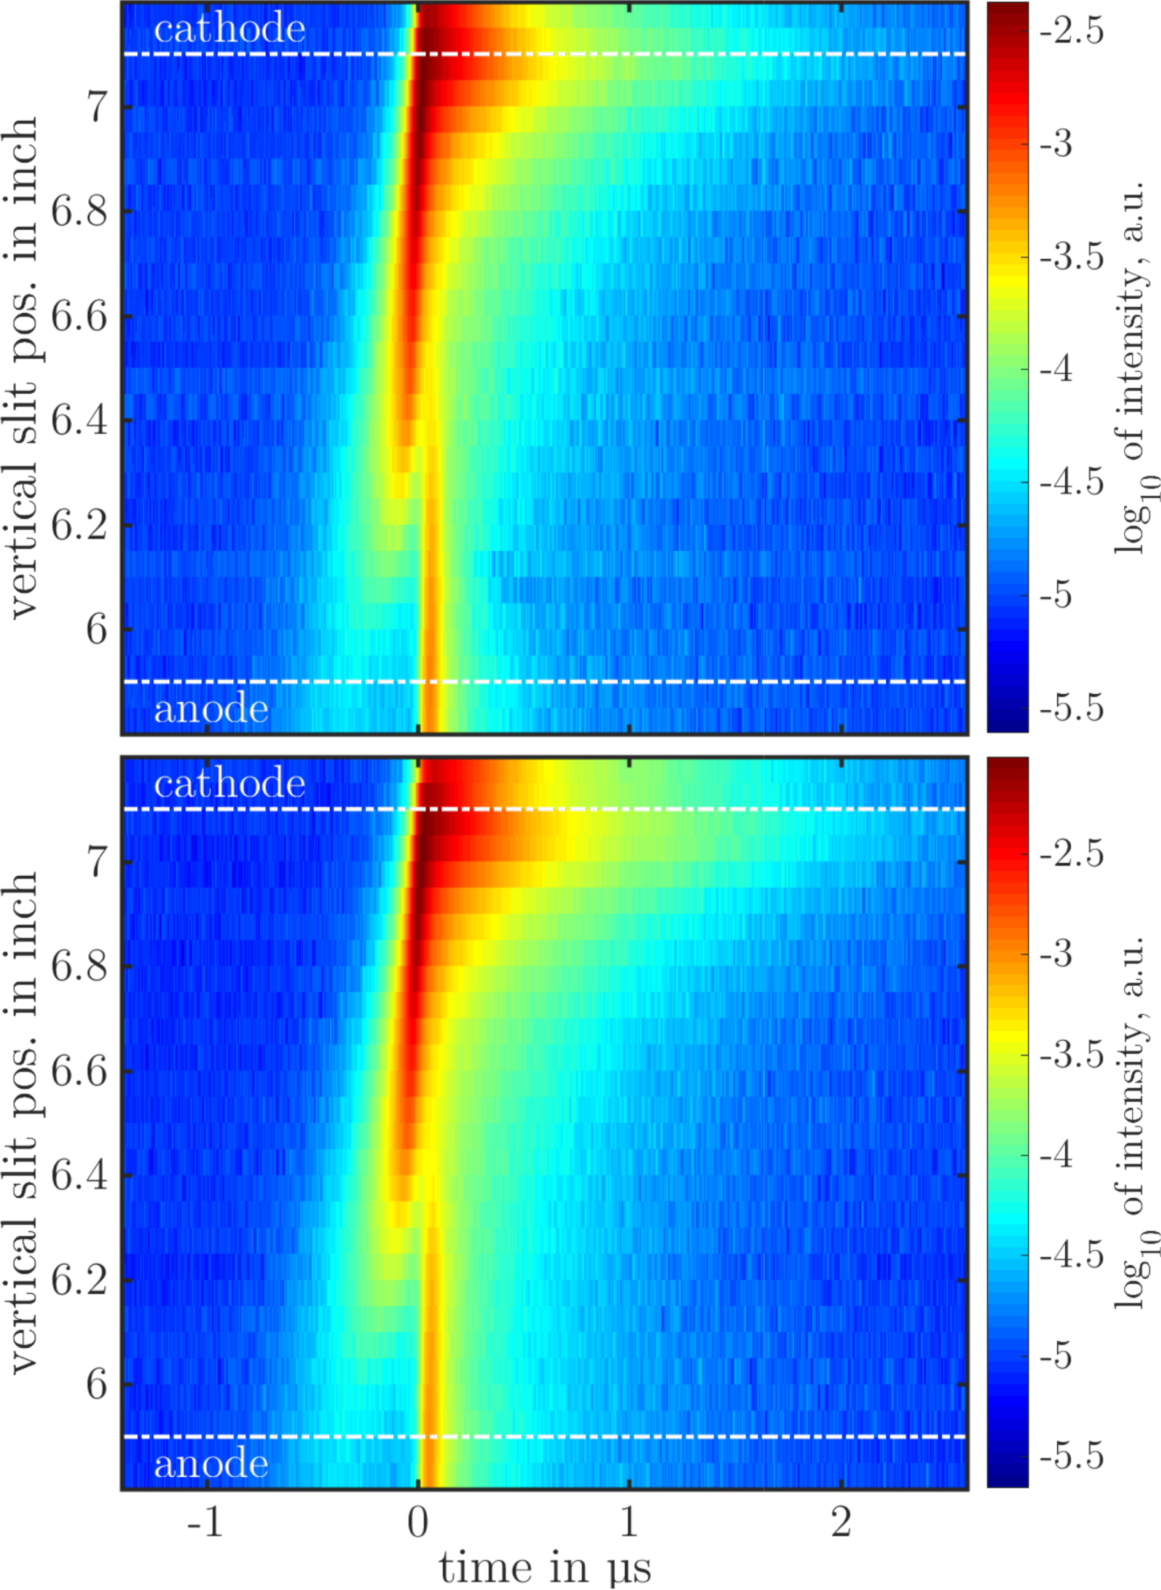
\includegraphics[width=\textwidth]{figures/lineratio/728u587.pdf}
					\caption*{}
					\label{img:728u587nm}
				\end{subfigure}
				\caption{\fett{(a)}: Spatio-temporally resolved line emission profiles for $\unit[667,98]{nm}$ (top) and $\unit[706,66]{nm}$ (bottom). \fett{(b)}: At $\unit[728,31]{nm}$ (top) and $\unit[587,65]{nm}$ (bottom). The discharge properties can be collected from \autoref{img:comparisonsinesquare}, as they happen to be the same experiments.}
				\label{img:comparisonemissionline}
			\end{figure}
			
			\begin{multicols}{2}
				
				\subsection{Electric field strength measurement by He I line emission ratios}
				
				
				
			\end{multicols}
			
			\twocolumn
		
		\subsection{Electric field strength measurement by stark spectroscopy}
		
				\begin{figure}[h]
					\centering
					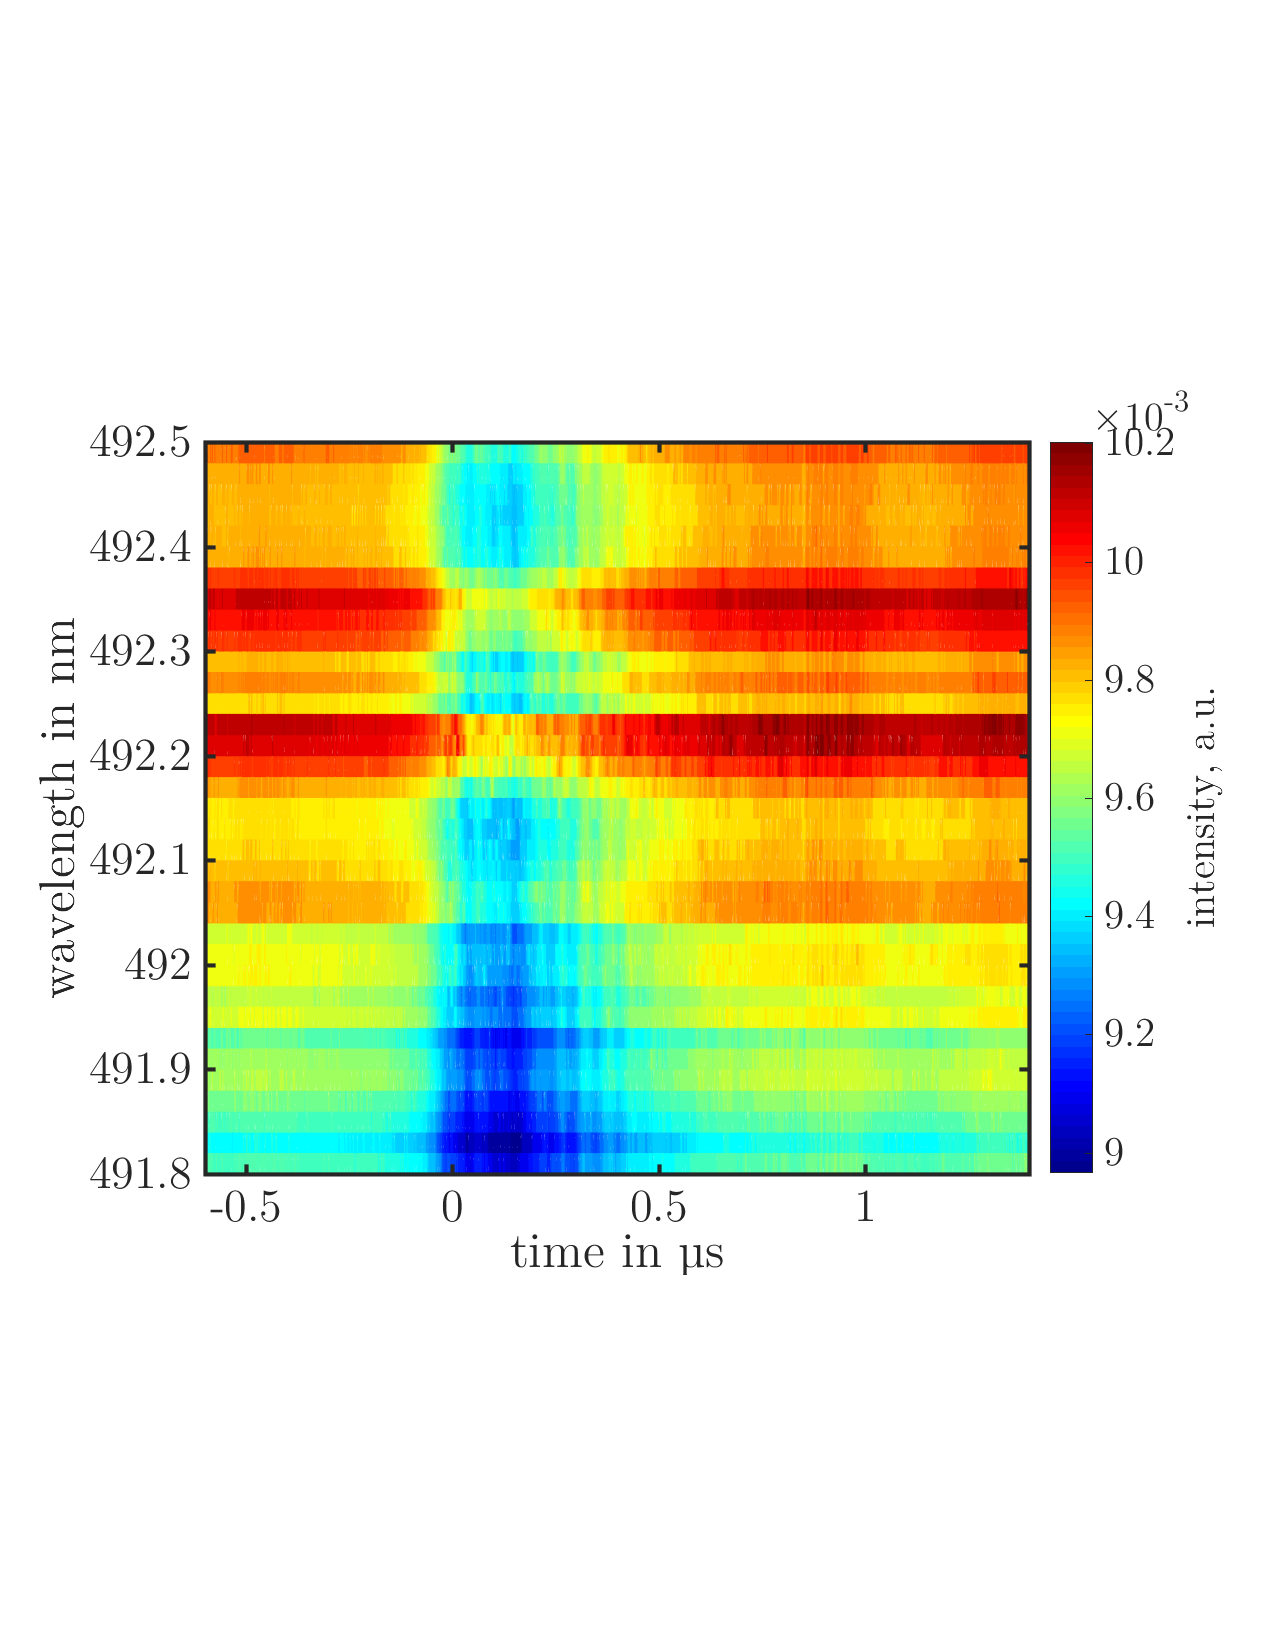
\includegraphics[width=0.5\textwidth]{figures/stark/stark_71inraw.pdf}
					\caption{Raw data from the temporally resolved stark spectroscopy at a vertical position of $\unit[7,1]{inch}$. The gathered information have not been processed any further, as only to be displayed here.}
				\end{figure}

				\begin{figure}
					\centering
					%\begin{subfigure}[t]{0.5\textwidth}
						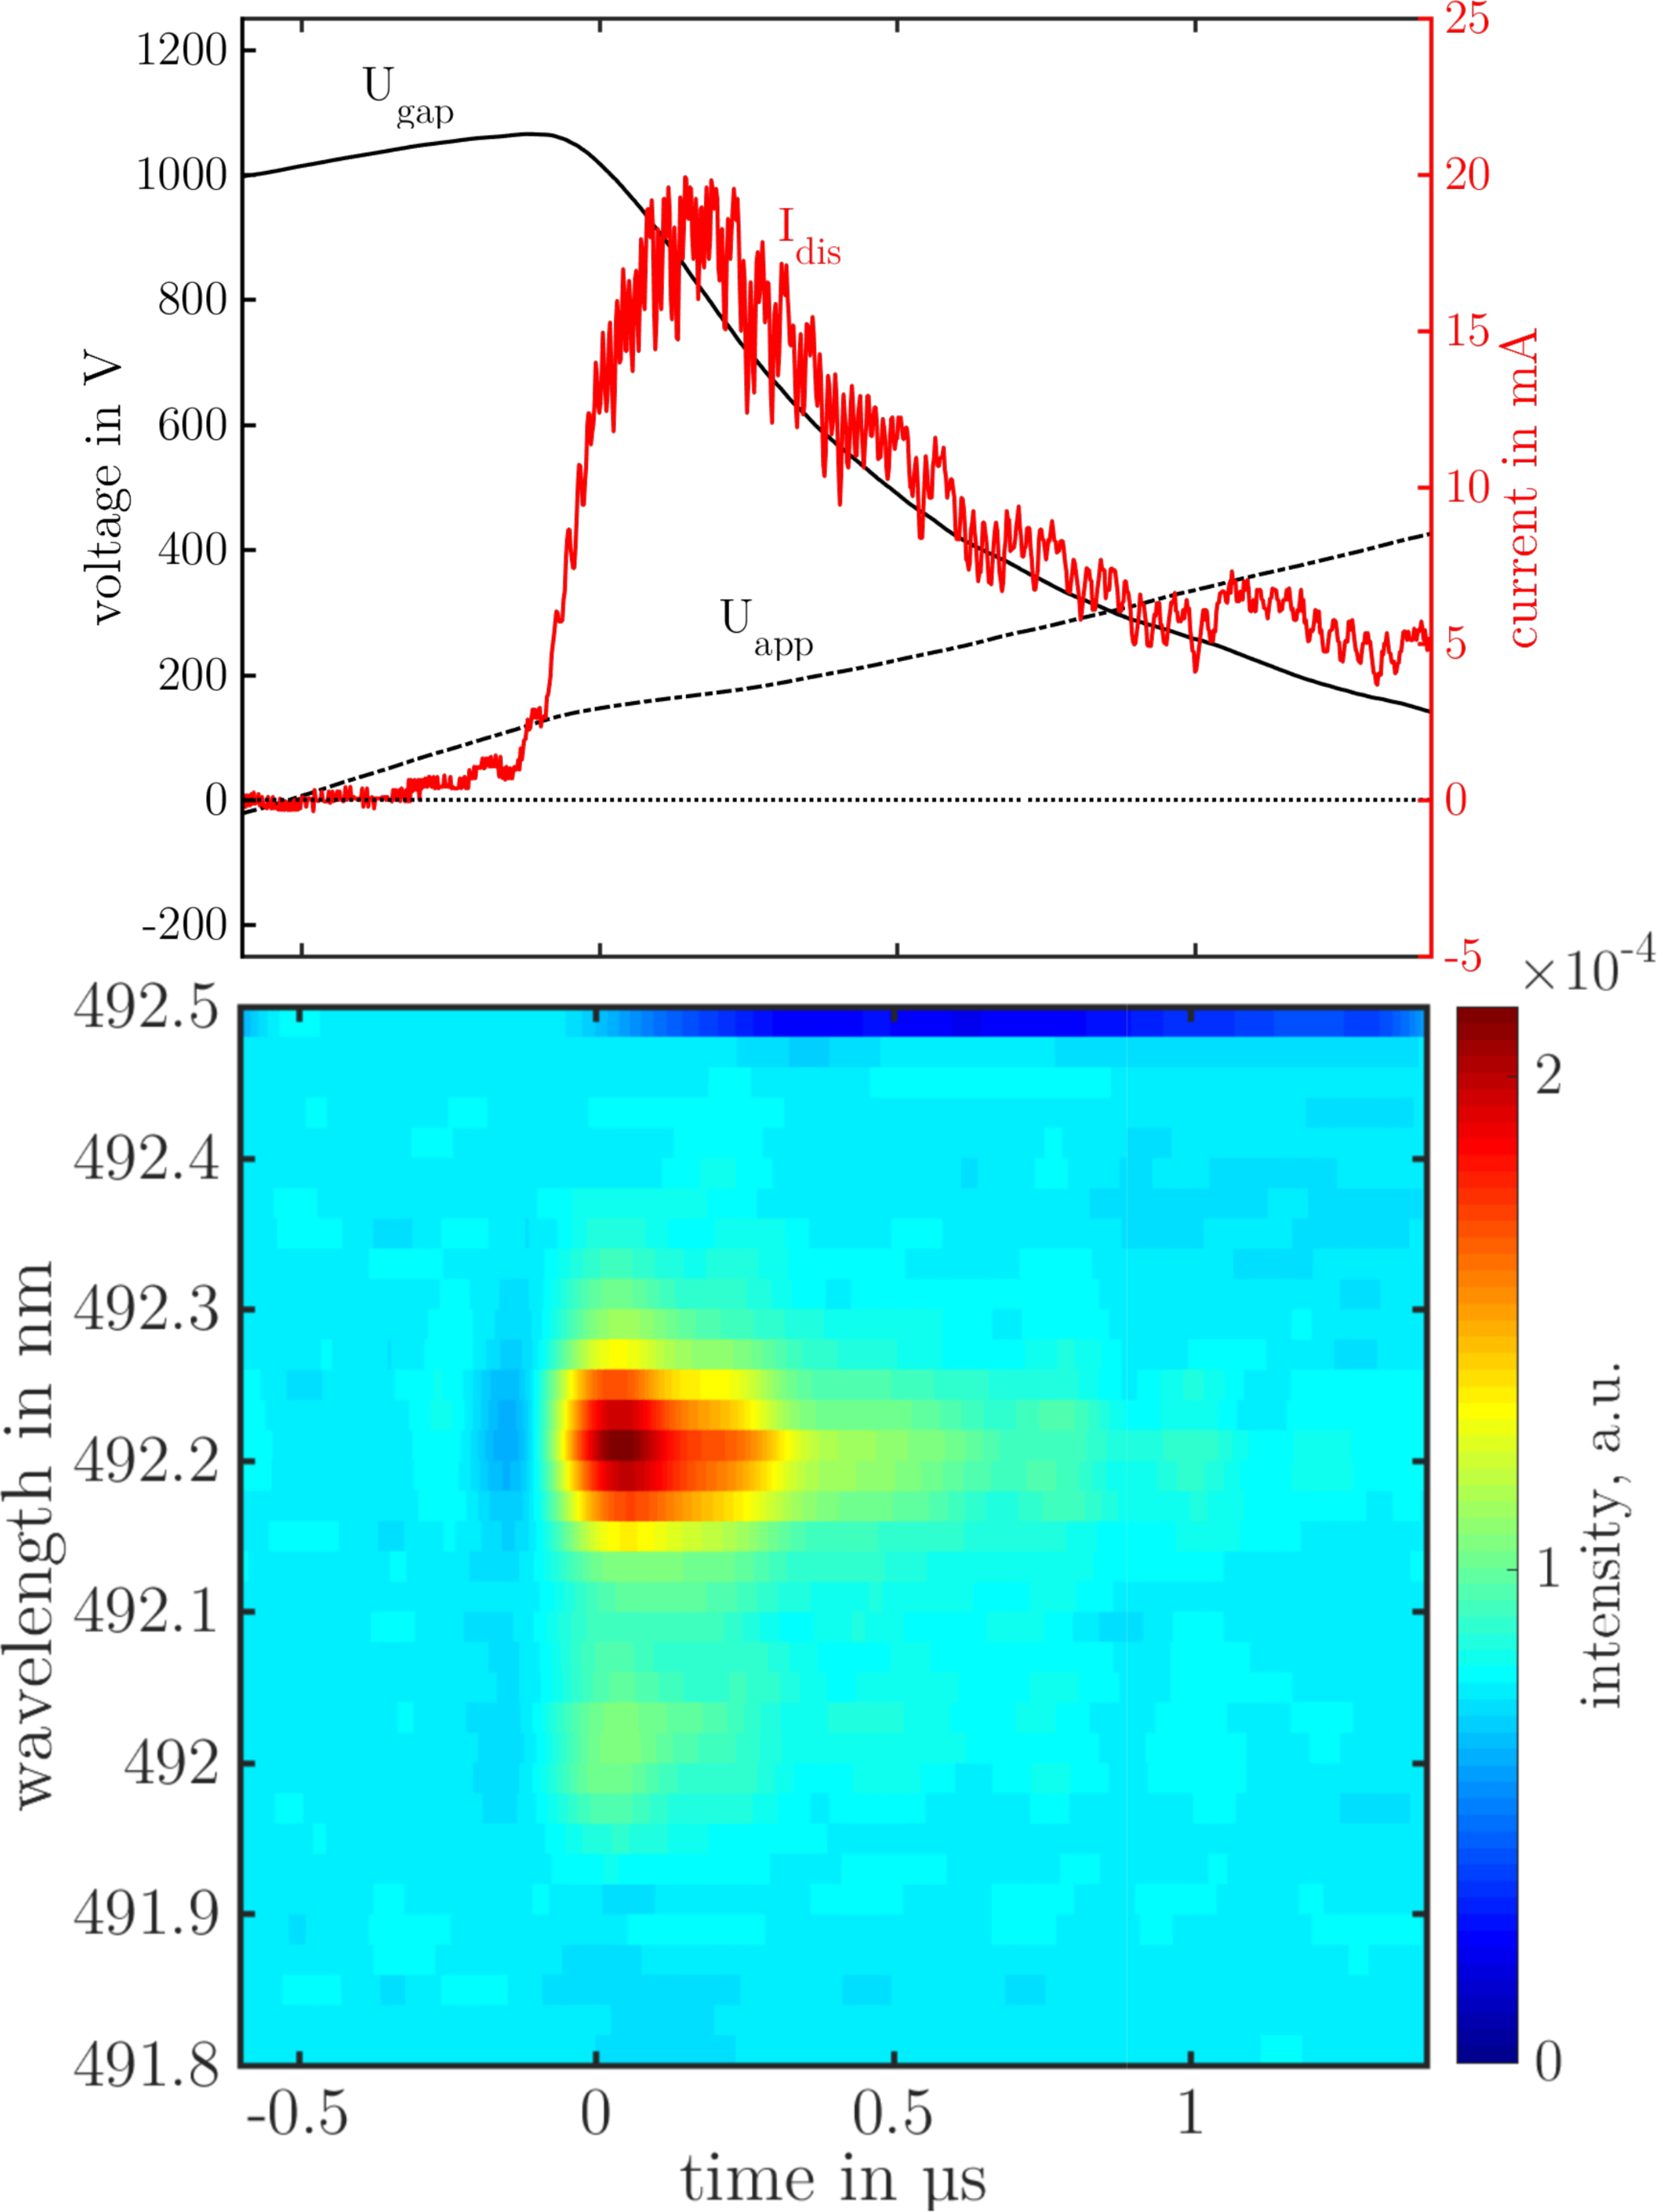
\includegraphics[width=0.5\textwidth]{figures/stark/stark71combination.pdf}
					%\end{subfigure}
					%\begin{subfigure}[b]{0.5\textwidth}
						%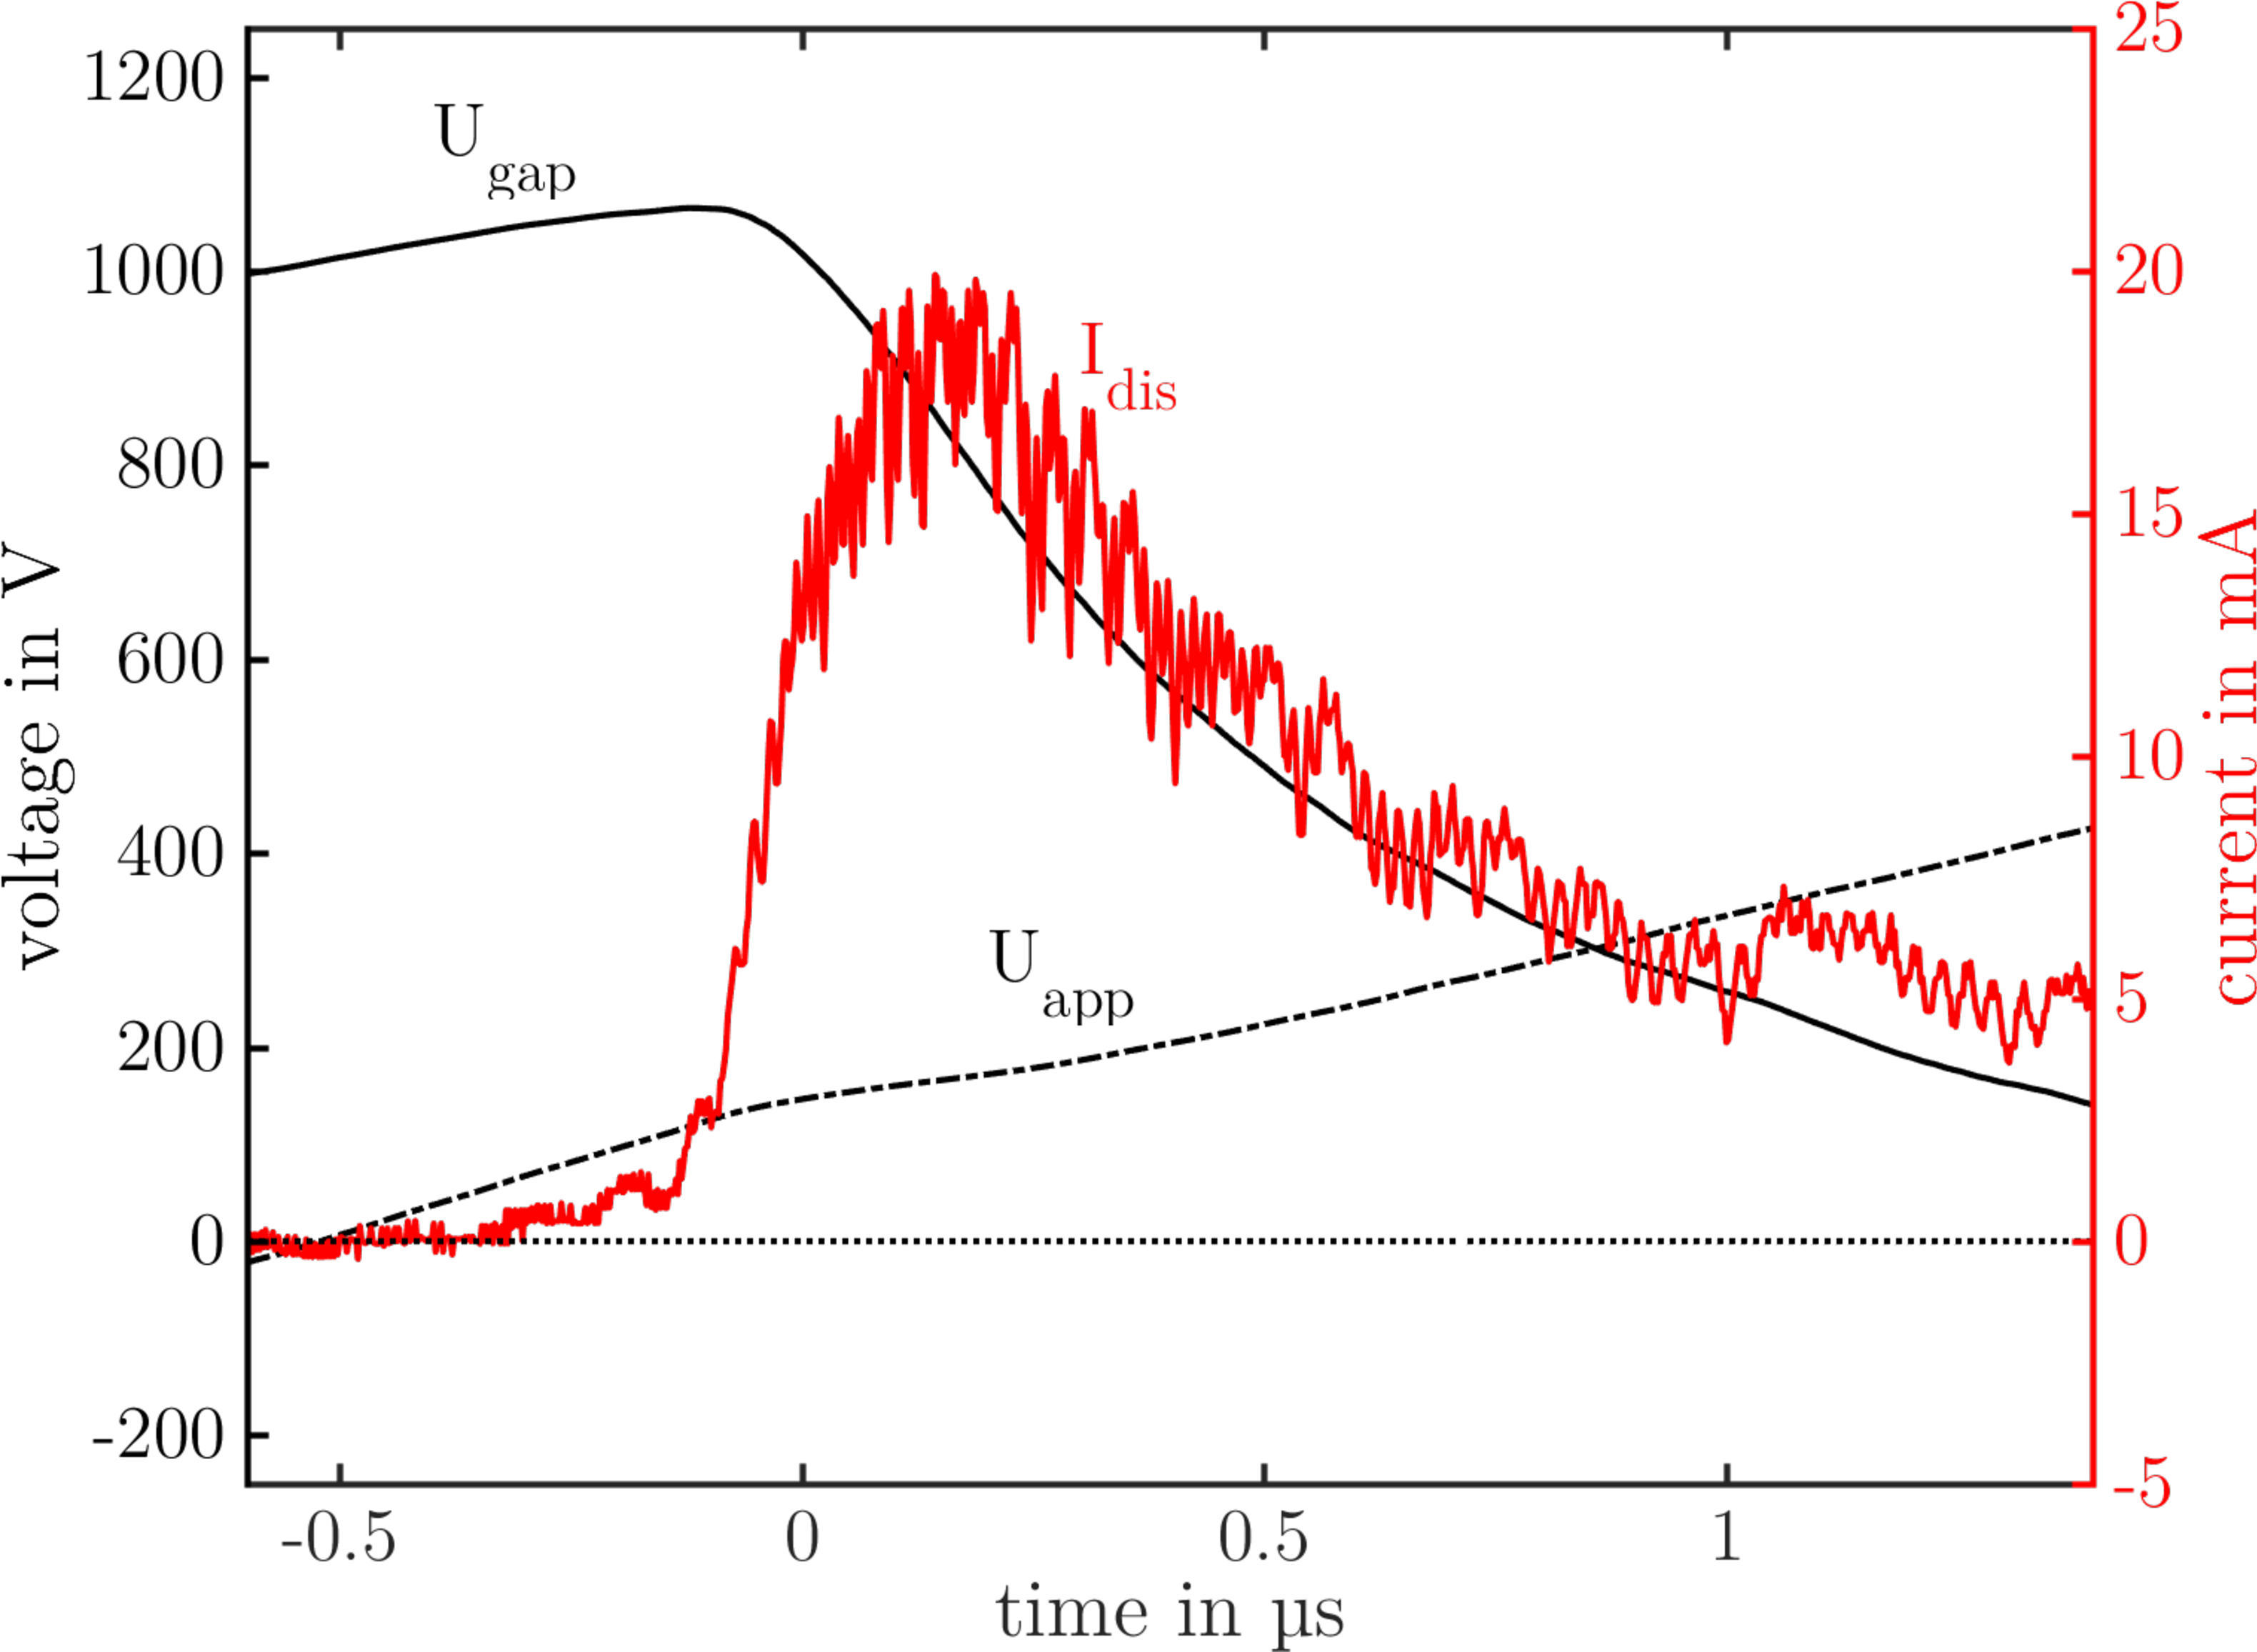
\includegraphics[width=\textwidth]{figures/stark/currentdis71.pdf}
					%\end{subfigure}
					\caption{Comparison of the dicharge properties and spectral emission during stark spectroscopy at a vertical position of $\unit[7,1]{inch}$. }
					\label{img:stark71comparison}
				\end{figure}

				\begin{figure}
					\centering
					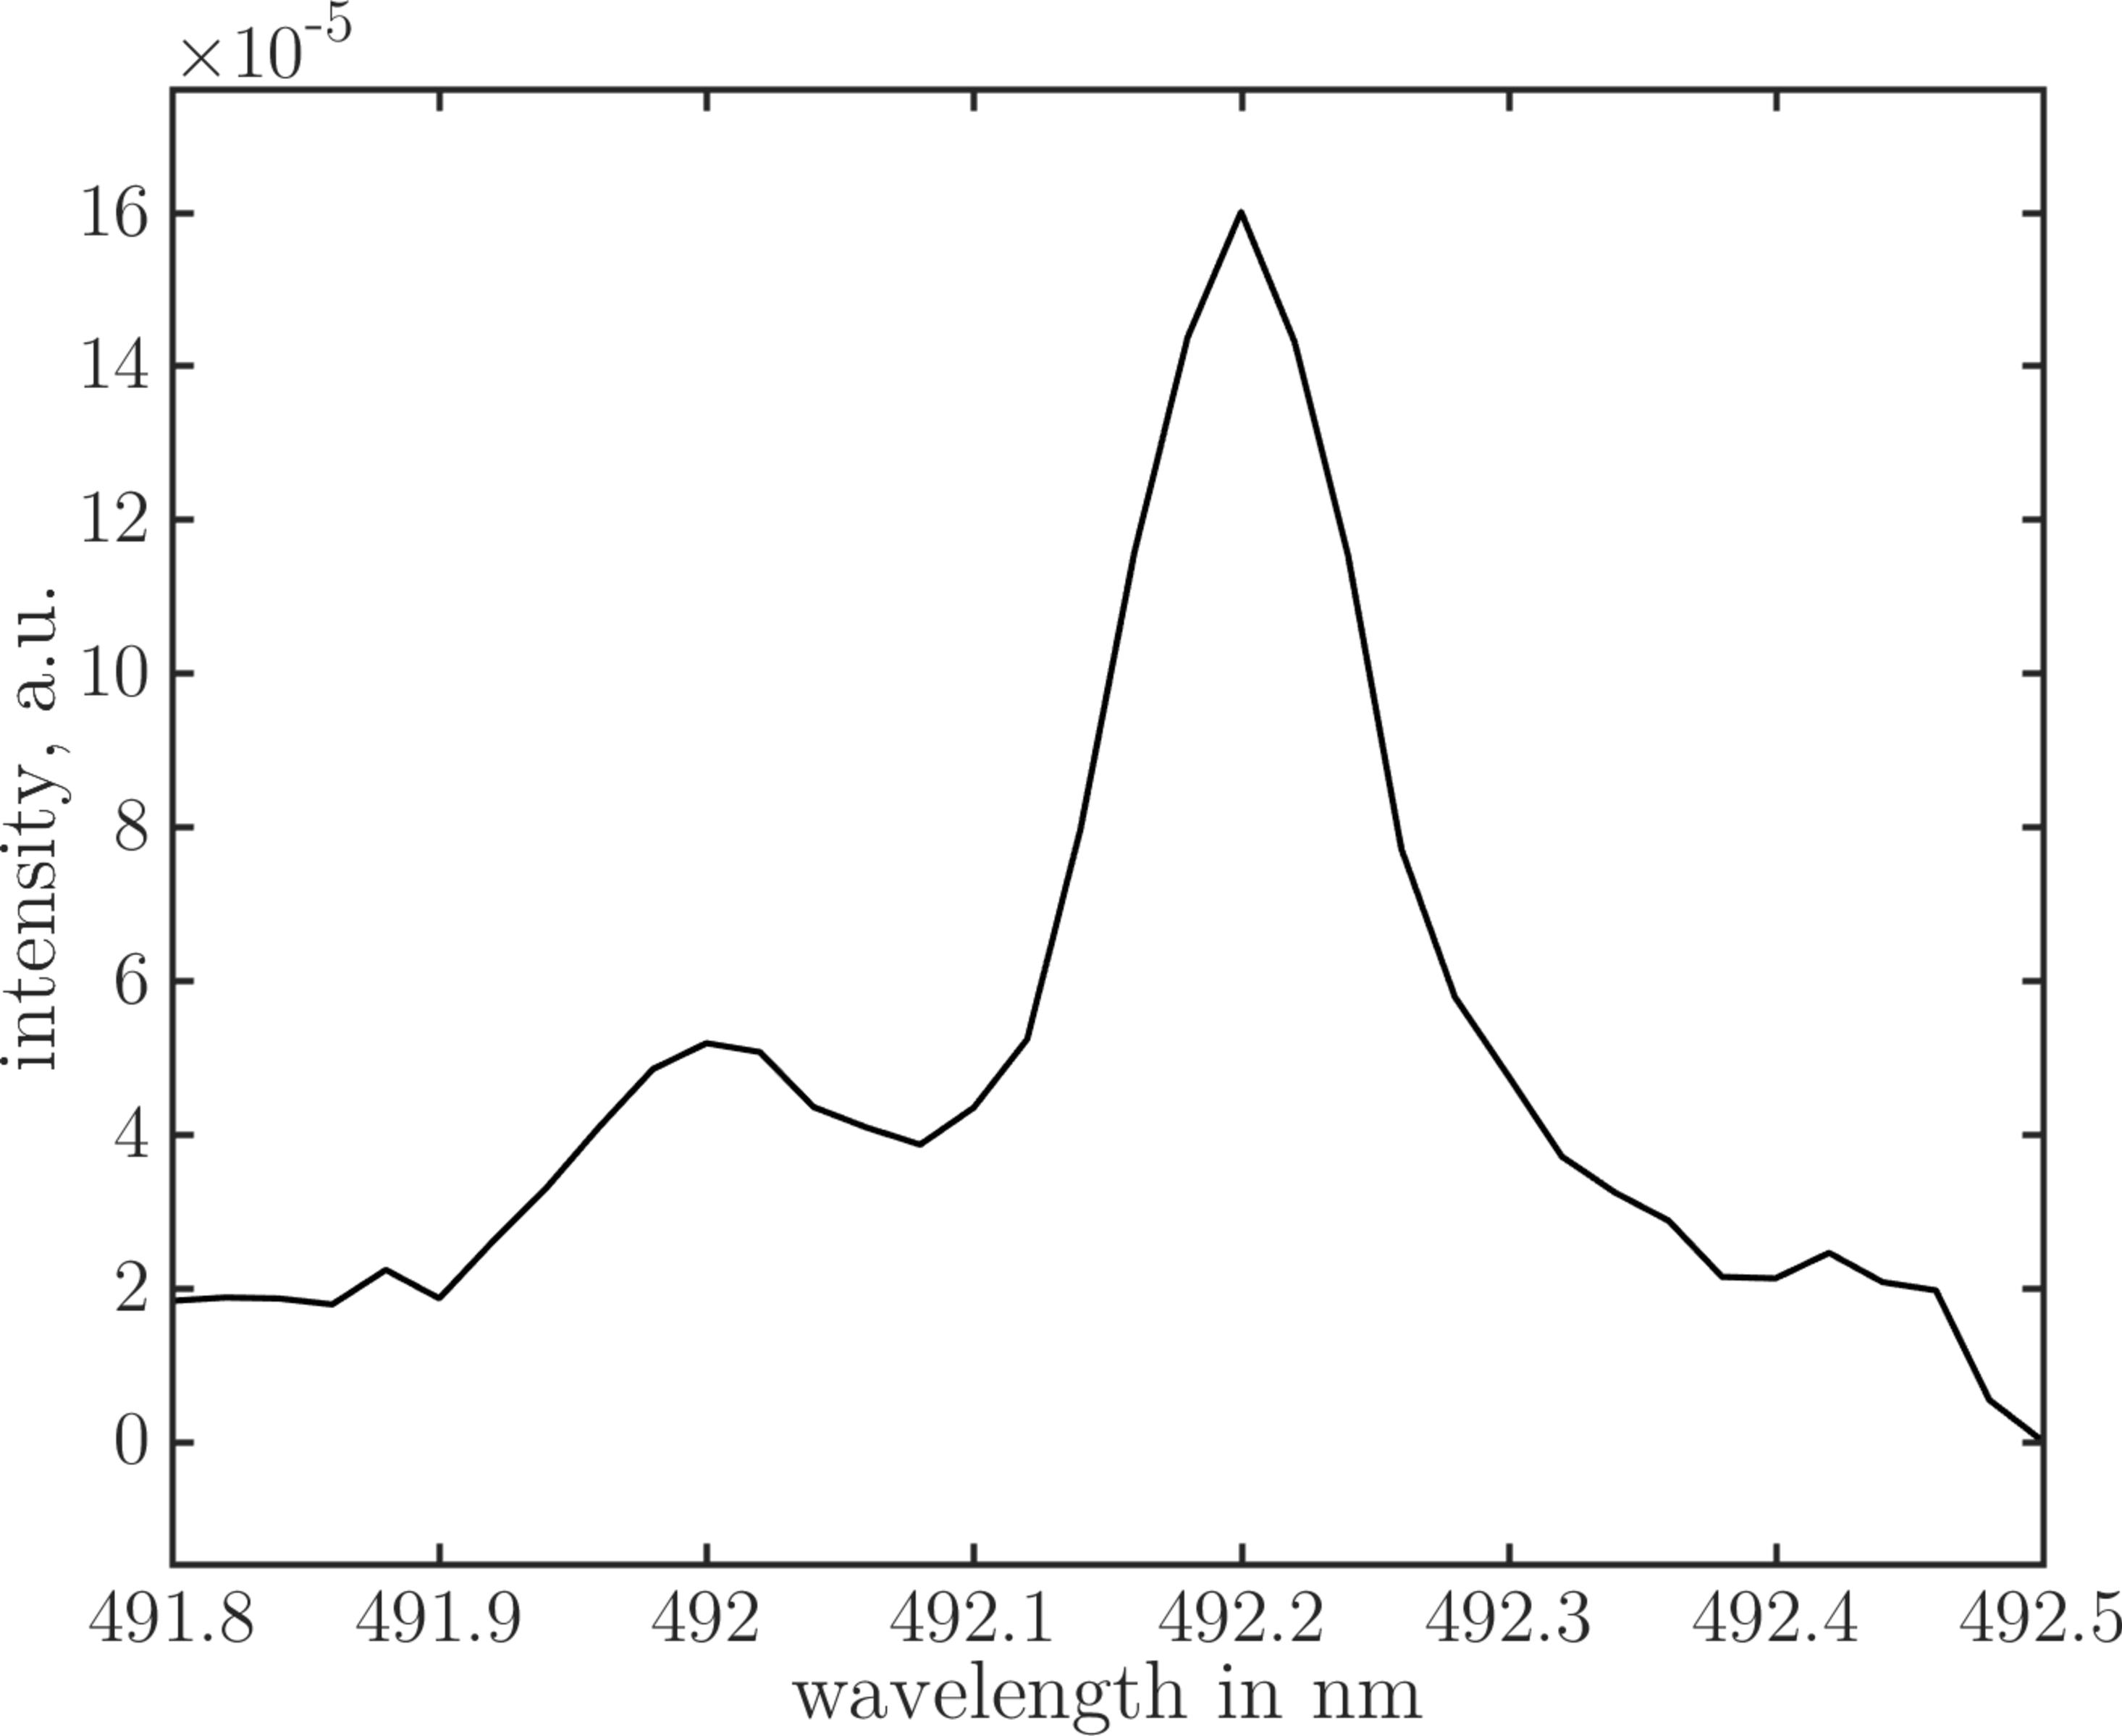
\includegraphics[width=0.5\textwidth]{figures/stark/stark_shift71in.pdf}
					\caption{Extracted emission profile around $\unit[492,2]{nm}$. This is at a relative time of $\unit[0,074]{\mu s}$ to the discharges ignition at $\unit[0]{\mu s}$.}
					\label{img:starkshift71}
				\end{figure}

		\subsection{Summary and outlook}
		
	\section{Literature}

		\bibliography{report.bib}
		\bibliographystyle{plain}
		
	\section{Appendix}


\end{document}